% ===================================================================
% O PRINCÍPIO DO CAJUEIRO
% Geometria de Contato e Aplicações (como quantificar, precificar, e priorizar a vida em sistemas vivos)
%
% Pablo Nogueira Grossi — G6 LLC, Newark, Nova Jersey
% Apresentação: XII Bienal de Matemática · SBM · UFRN, Natal · Agosto 2026
%
% Monografia completa, ~120 páginas, estilo da monografia de matéria escura.
% ===================================================================

\documentclass[12pt,a4paper,twoside]{book}

\usepackage[utf8]{inputenc}
\usepackage[T1]{fontenc}
\usepackage{lmodern}          % heavier, crisper Latin Modern fonts
\setlength{\headheight}{14pt} % suppress fancyhdr warning
% babel-portuguese not installed in this environment; manual renaming below
\renewcommand{\chaptername}{Capítulo}
\renewcommand{\partname}{Parte}
\renewcommand{\appendixname}{Apêndice}
\renewcommand{\contentsname}{Sumário}
\renewcommand{\bibname}{Bibliografia}
\renewcommand{\listfigurename}{Lista de Figuras}
\renewcommand{\listtablename}{Lista de Tabelas}
\renewcommand{\figurename}{Figura}
\renewcommand{\tablename}{Tabela}
\renewcommand{\indexname}{Índice Remissivo}
\usepackage[margin=1in]{geometry}
\usepackage{amsmath,amssymb,amsthm,amsfonts,mathtools}
\usepackage{graphicx,xcolor}
\usepackage{hyperref}
\usepackage{booktabs}
\usepackage{enumitem}
\usepackage[final,expansion=false]{microtype}
\usepackage{listings}
\usepackage{fancyhdr}
\usepackage{titlesec}
\usepackage{tocbibind}
\usepackage[most]{tcolorbox}   % callout boxes
\tcbset{fonttitle=\bfseries}
\usepackage{epigraph}
\usepackage{tikz}
\usetikzlibrary{arrows.meta,decorations.pathmorphing,shapes.geometric,positioning,calc}

\hypersetup{
  colorlinks=true,
  linkcolor=blue!50!black,
  urlcolor=blue!60!black,
  citecolor=blue!40!black,
  pdftitle={O Princípio do Cajueiro — Geometria de Contato e Aplicações (como quantificar, precificar, e priorizar a vida em sistemas vivos)},
  pdfauthor={Pablo Nogueira Grossi}
}

\definecolor{cajugold}{rgb}{0.79,0.66,0.30}
\definecolor{cajunavy}{rgb}{0.10,0.16,0.27}
\definecolor{cajured}{rgb}{0.55,0.20,0.20}
\definecolor{codebg}{rgb}{0.97,0.97,0.97}
\definecolor{kw}{rgb}{0.0,0.0,0.6}
\definecolor{str}{rgb}{0.6,0.0,0.0}
\definecolor{cmt}{rgb}{0.2,0.5,0.2}

\lstdefinelanguage{lean}{
  keywords={import,namespace,open,def,axiom,lemma,theorem,corollary,by,exact,apply,intro,intros,have,show,use,let,fun,if,then,else,match,with,rfl,sorry,push_neg,linarith,norm_num,positivity,unfold,split_ifs,split,cases,constructor,refine,end},
  sensitive=true,
  morecomment=[l]{--},
  morecomment=[s]{/-}{-/},
  morestring=[b]"
}

\lstset{
  basicstyle=\ttfamily\small,
  backgroundcolor=\color{codebg},
  keywordstyle=\color{kw}\bfseries,
  stringstyle=\color{str},
  commentstyle=\color{cmt}\itshape,
  showstringspaces=false,
  breaklines=true,
  frame=single,
  rulecolor=\color{black!20},
  numbers=left,
  numberstyle=\tiny\color{black!50},
  numbersep=8pt
}

\theoremstyle{plain}
\newtheorem{teorema}{Teorema}[section]

% ── Claim-type environments ──────────────────────────────────────────
% PROVADO  — mathematically proved with formal proof
% TEORIZADO — physically motivated framework, not yet experimentally confirmed
% CONJECTURA — speculative, open programme

\theoremstyle{definition}
\newtheorem{hipotese}{Hipótese}[section]   % theorized claim

\newcommand{\provadostamp}{\noindent\colorbox{cajunavy!10}{\color{cajunavy}\bfseries\small PROVADO}\quad}
\newcommand{\teorizadostamp}{\noindent\colorbox{cajugold!20}{\color{cajugold!60!black}\bfseries\small TEORIZADO}\quad}
\newcommand{\conjecturastamp}{\noindent\colorbox{cajured!10}{\color{cajured}\bfseries\small CONJECTURA}\quad}
\renewcommand{\proofname}{Demonstração}
\newtheorem{lema}[teorema]{Lema}
\newtheorem{proposicao}[teorema]{Proposição}
\newtheorem{corolario}[teorema]{Corolário}

\theoremstyle{definition}
\newtheorem{definicao}[teorema]{Definição}
\newtheorem{exemplo}[teorema]{Exemplo}
\newtheorem{observacao}[teorema]{Observação}
\newtheorem{conjectura}[teorema]{Conjectura}
\newtheorem{contraexemplo}[teorema]{Contraexemplo}

\renewcommand{\headrulewidth}{0.4pt}
\pagestyle{fancy}
\fancyhf{}
\fancyhead[LE,RO]{\thepage}
\fancyhead[RE]{\itshape\nouppercase{\leftmark}}
\fancyhead[LO]{\itshape\nouppercase{\rightmark}}

\titleformat{\chapter}[display]{\normalfont\Large\bfseries\color{cajunavy}}{\partname\ \thechapter}{14pt}{\Huge}

\setlength{\epigraphwidth}{0.55\textwidth}
\renewcommand{\epigraphsize}{\small}
\renewcommand{\epigraphflush}{flushright}

\newcommand{\R}{\mathbb{R}}
\newcommand{\C}{\mathbb{C}}
\newcommand{\N}{\mathbb{N}}
\newcommand{\Z}{\mathbb{Z}}
\newcommand{\eps}{\varepsilon}
\newcommand{\epsz}{\varepsilon_{0}}
\newcommand{\tribo}{\eta}
\newcommand{\Reeb}{R_\alpha}
\newcommand{\Lie}{\mathcal{L}}
\newcommand{\dd}{\mathrm{d}}
\newcommand{\dm}{\mathrm{dm}^{3}}

\title{
  \vspace{-2cm}
  \rule{\textwidth}{1.5pt}\\[0.5cm]
  {\Huge\bfseries\color{cajunavy} O Princípio do Cajueiro}\\[0.4cm]
  {\Large Geometria de Contato e Aplicações}\\[0.2cm]
  {\normalsize\itshape como quantificar, precificar, e priorizar a vida em sistemas vivos}\\[0.6cm]
  \rule{\textwidth}{1.5pt}\\[1.2cm]
  {\large Uma Monografia Completa}\\[0.3cm]
  {\normalsize Apresentação na XII Bienal de Matemática}\\
  {\normalsize Sociedade Brasileira de Matemática · UFRN · Natal/RN}\\
  {\normalsize Agosto de 2026}
}

\author{
  \large Pablo Nogueira Grossi\thanks{G6~LLC, Newark, Nova Jersey 07104, EUA.
  ORCID: 0009-0000-6496-2186. Correio eletrônico: \texttt{g6llc@proton.me}.
  Telefone: +1 (646) 342-3751.}\\
  \normalsize G6 LLC, Newark, Nova Jersey
}
\date{Junho de 2026}

\begin{document}
\frontmatter
\maketitle

% ── Cover diagram ───────────────────────────────────────────────────
\thispagestyle{empty}
\vspace{1cm}
\begin{center}
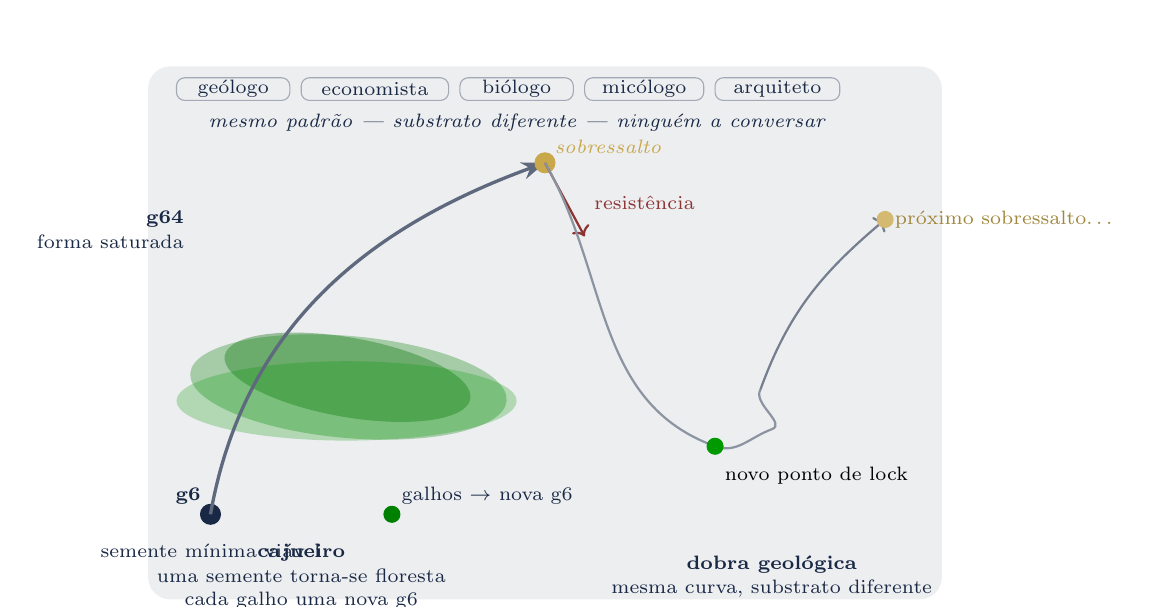
\begin{tikzpicture}[scale=0.72, every node/.style={font=\scriptsize}]
  \fill[cajunavy!8, rounded corners=8pt] (-0.5,-1.2) rectangle (13.5,8.2);
  % Discipline chips — individually sized
  \draw[cajunavy!40, rounded corners=3pt] (0.0,7.6) rectangle (2.0,8.0);
  \node[cajunavy] at (1.0,7.8) {geólogo};
  \draw[cajunavy!40, rounded corners=3pt] (2.2,7.6) rectangle (4.8,8.0);
  \node[cajunavy] at (3.5,7.8) {economista};
  \draw[cajunavy!40, rounded corners=3pt] (5.0,7.6) rectangle (7.0,8.0);
  \node[cajunavy] at (6.0,7.8) {biólogo};
  \draw[cajunavy!40, rounded corners=3pt] (7.2,7.6) rectangle (9.3,8.0);
  \node[cajunavy] at (8.25,7.8) {micólogo};
  \draw[cajunavy!40, rounded corners=3pt] (9.5,7.6) rectangle (11.7,8.0);
  \node[cajunavy] at (10.6,7.8) {arquiteto};
  \node[align=center, cajunavy] at (6.0, 7.2)
    {\itshape mesmo padrão --- substrato diferente --- ninguém a conversar};
  % Cajueiro canopy
  \fill[green!40!black, opacity=0.35, rotate=-10] (2.5,3.2) ellipse (2.2cm and 0.7cm);
  \fill[green!50!black, opacity=0.30, rotate=-5]  (2.8,2.8) ellipse (2.8cm and 0.9cm);
  \fill[green!60!black, opacity=0.25]              (3.0,2.3) ellipse (3.0cm and 0.7cm);
  % g6 seed
  \filldraw[cajunavy] (0.6,0.3) circle (5pt);
  \node[above left, cajunavy] at (0.6,0.3) {\normalfont\bfseries g6};
  \node[below, cajunavy, align=center] at (0.6,-0.05)
    {semente mínima viável};
  % g64 label
  \node[left, cajunavy] at (0.3, 5.5) {\normalfont\bfseries g64};
  \node[left, cajunavy] at (0.3, 5.1) {forma saturada};
  % Branch root dot
  \filldraw[green!50!black] (3.8,0.3) circle (4pt);
  \node[above right, cajunavy] at (3.8,0.3) {galhos $\to$ nova g6};
  % Main arc: g6 → overshoot
  \draw[cajunavy!70, very thick, ->, >=Stealth]
    (0.6,0.3) to[out=80, in=200] (6.5,6.5);
  \filldraw[cajugold] (6.5,6.5) circle (5pt);
  \node[above right] at (6.5,6.5) {\textcolor{cajugold}{\itshape sobressalto}};
  % Resistance
  \draw[cajured, thick, ->] (6.5,6.5) -- (7.2,5.2);
  \node[right, cajured] at (7.2, 5.8) {resistência};
  % Fold curve
  \draw[cajunavy!50, thick] (6.5,6.5) to[out=-60, in=160] (9.5,1.5)
    to[out=-20, in=200] (10.5,1.8) to[out=20, in=240] (10.3,2.5);
  \filldraw[green!60!black] (9.5,1.5) circle (4pt);
  \node[below right] at (9.5,1.3) {novo ponto de lock};
  % Next overshoot
  \draw[cajunavy!60, thick, ->] (10.3,2.5) to[out=70, in=220] (12.5,5.5);
  \filldraw[cajugold!80] (12.5,5.5) circle (4pt);
  \node[right] at (12.5,5.5) {\textcolor{cajugold!80!black}{próximo sobressalto\ldots}};
  % Bottom captions — clear of dots
  \node[align=center, cajunavy] at (2.2,-0.8)
    {\normalfont\bfseries cajueiro\\[1pt]uma semente torna-se floresta\\cada galho uma nova g6};
  \node[align=center, cajunavy] at (10.5,-0.8)
    {\normalfont\bfseries dobra geológica\\[1pt]mesma curva, substrato diferente};
\end{tikzpicture}

\vspace{0.4cm}
{\small\color{cajunavy}\itshape
g6: semente mínima viável \quad|\quad g64: forma saturada \quad|\quad
cada galho, uma nova g6 --- cada nova g6, uma nova floresta}
\end{center}
\newpage

% ──────────────────────────────────────────────────────────────────
\chapter*{Resumo}
\addcontentsline{toc}{chapter}{Resumo}

Esta monografia apresenta o \textbf{Princípio do Cajueiro} --- uma estrutura
contato-geométrica para transições generativas. As afirmações são classificadas
em três categorias epistêmicas, mantidas rigorosamente separadas ao longo do
texto:

\medskip
\begin{center}
\begin{tabular}{lp{9cm}}
\colorbox{cajunavy!10}{\color{cajunavy}\bfseries\small PROVADO} &
  Afirmações com prova matemática formal (verificadas em Lean~4 ou
  demonstradas rigorosamente no texto). \\[4pt]
\colorbox{cajugold!20}{\color{cajugold!60!black}\bfseries\small TEORIZADO} &
  Afirmações com motivação física sólida e estrutura matemática, mas
  ainda não confirmadas experimentalmente como instâncias do arcabouço dm$^{3}$. \\[4pt]
\colorbox{cajured!10}{\color{cajured}\bfseries\small CONJECTURA} &
  Afirmações especulativas que constituem programa de pesquisa aberto. \\
\end{tabular}
\end{center}

\bigskip
\noindent\textbf{\large O que provamos}

\smallskip
\provadostamp
A cadeia de operadores de contato $G = U \circ F \circ K \circ C$
é \emph{bem-posta} e \emph{não-comutativa} sob hipóteses explícitas
(Teoremas 3.6.1--3.6.2). A não-comutatividade $[K,F]\ne 0$ é o mecanismo
formal que distingue as duas ordens catalíticas.

\provadostamp
As constantes $\epsz = 1/3$ (raio de Gronwall), $\tau = 2$ (limiar de
convergência) e $\tribo \approx 1{,}839$ (constante de Tribonacci) são
\emph{derivadas}, não ajustadas, a partir do modelo $\dm$
(Teoremas 5.2.2, 4.2.1, 5.3.2). Todas estão certificadas em Lean~4.

\provadostamp
As singularidades de Whitney de codimensão $\le 3$ são completamente
classificadas (Teorema~A); uma dobra $A_1$ sobre $\Sigma$ corresponde
bijetivamente a uma órbita fechada de Reeb em $M$ (Teorema~B); a
forma simplética é preservada a menos de fator conforme (Teorema~C);
o modelo $\dm$ possui atrator global $\Gamma = \{r=1\}$ (Teorema~D).

\provadostamp
\textbf{Teoremas Cajueiro C1--C7:}
(C5)~a corda é estritamente mais curta que o arco em $S^{3}$, com razão mínima
$2/\pi$ no caso antipodal;
(C7)~a ascendência ao limiar $\eta$-ponderada $\sum_{k}\eta^{-k} = \eta/(\eta-1)$ converge
a $\tau = 2$ quando $\eta \to 2$, e excede $\eta$ para todo $\eta \in (1,2)$;
(C2)~se $d_O/d_I > 10$, necessariamente existe mecanismo de inflação do meio
(prova por contradição via desigualdade de processamento de dados).

\bigskip
\noindent\textbf{\large O que teorizamos}

\smallskip
\teorizadostamp
Propõe-se que o índice de ordem de operadores $O = t_{\mathrm{DEE}}/t_{\mathrm{EtO}}$
(medido por DRIFTS) distingue os regimes ZSM-5 e MCM-22 porque a topologia
do poro impõe uma \emph{ordem} aos operadores da cadeia $G$
(Hipótese~10.2.1). Esta interpretação é \emph{consistente} com os
dados experimentais de \cite{Sousa2014,Sousa2023} e com a não-comutatividade
provada; não é derivada a partir deles.

\teorizadostamp
As três instâncias físicas --- criovulcanismo de Encélado
\cite{Khawaja2025}, ventos hidrotermais alcalinos \cite{Russell,Sojo}
e auto-replicação ribozímica \cite{Joyce} --- são \emph{consistentes}
com a estrutura de operadores $G = U \circ F \circ K \circ C$. Não
afirmamos que a cadeia $G$ \emph{seja} o mecanismo desses sistemas;
afirmamos que ela os descreve sem contradição e com poder preditivo.

\teorizadostamp
A interpretação do fóton como portador de um elemento de contato
$(q_0, \hbar\mathbf{k}_0, (\ell+\sigma)\hbar)$ (Teorema~C1) é
formalmente correta em óptica quântica paraxial. A extensão ao
sinalamento biológico (rodopsina, fotorreceptores) é uma
\emph{hipótese} motivada pela geometria, não um resultado
experimental.

\teorizadostamp
A ``ortogênese topológica'' --- a direcionalidade das transições
generativas como propriedade do espaço de fases, não dos sistemas
--- é uma re-interpretação consistente com a geometria de contato.
Ela \emph{não substitui} a biogênese química; ela propõe que
a geometria de fase é uma camada adicional de estrutura.

\bigskip
\noindent\textbf{\large O que conjecturamos}

\smallskip
\conjecturastamp
Que as transições generativas em \emph{todos} os sistemas físicos,
biológicos e industriais formam uma única \textbf{classe de universalidade}
definida pela álgebra de $G$ --- i.e., que a cadeia $C \to K \to F \to U$
é o esqueleto universal de toda transição generativa. Isso vai além do
que foi provado ou verificado experimentalmente.

\conjecturastamp
Que a geometria $S^{3}/H^{4}$ (3-esfera como fronteira do hiperplano
generativo $H^4$) descreve o espaço de fase das transições generativas
em geral. A equidistância generativa $G^{*}d = 0$ (Teorema~C4) é
formalmente correta em $S^3$; sua aplicação a sistemas físicos é
conjectural.

\conjecturastamp
Que o Cajueiro de Pirangi --- e o Kalpataru da tradição indiana ---
realizam literalmente o Princípio do Cajueiro: que o mecanismo de
expansão clonal via raízes aéreas instancia a cadeia $G$ em escala
biológica. Esta é uma analogia inspiradora, não uma prova.

\bigskip
\noindent \provadostamp As constantes canônicas $\epsz = 1/3$, $\tau = 2$,
$\tribo \approx 1{,}839$ são derivadas do modelo $\dm$ e certificadas em Lean~4.
Toda afirmação nesta monografia carrega um dos três selos acima.


% ── Note for the biologist / physician reader ───────────────────────
\begin{tcolorbox}[
  colback=cajunavy!5,
  colframe=cajunavy!40,
  title={Para o leitor biólogo, médico ou engenheiro químico},
  breakable
]

\textbf{Os teoremas nesta monografia são matemática.}
Eles afirmam que, dentro de um sistema formal específico --- uma variedade de
contato com operadores bem definidos --- certas propriedades se seguem
necessariamente. Um teorema é verdadeiro porque foi provado a partir de
axiomas, não porque observamos o fenômeno na natureza.

\medskip
\textbf{O que acontece na natureza é física.}
\teorizadostamp A afirmação de que o cajueiro de Pirangi, o criovulcanismo de
Encélado, ou o ribossoma \emph{realizam} a cadeia $G = U \circ F \circ K \circ C$
é uma hipótese física teórica não comprovada --- apesar de termos uma boa ideia
de que é o caminho certo. Ela diz que o sistema matemático é um bom modelo para
esses fenômenos. Modelos são testáveis e falsificáveis.
Onde o texto carrega apenas o selo \provadostamp, a afirmação é matemática pura.

\medskip
\textbf{O que é $\tau = 2$, em linguagem não-matemática?}
A sequência n-bonacci --- Fibonacci ($\varphi \approx 1{,}618$),
Tribonacci ($\eta \approx 1{,}839$), Tetranacci ($\Delta \approx 1{,}927$)
e assim por diante --- converge a um limite fixo quando o número de
termos na recorrência cresce sem limite. Esse limite é $\tau = 2$.
É o \emph{teto de amplificação} da ascendência ao limiar do cajueiro:
o ponto além do qual a razão entre o que a instrução mínima controla
e o que o meio entrega não pode crescer.

Para um médico: quando 1\,mg de adrenalina desencadeia uma resposta
fisiológica que mobiliza bilhões de células, a razão
instrução/resposta não é ilimitada --- ela tem um teto geométrico.
$\tau = 2$ é esse teto na geometria de contato. A bioquímica da
adrenalina (os receptores, as vias de AMPc, a fosforilação de
proteínas) é o mecanismo físico, que os fisiologistas descrevem.
A \emph{geometria} da amplificação --- o fato de que toda ascendência
(generativa) ao limiar tem o mesmo teto $\tau = 2$ --- é o que esta monografia prova.

Para um engenheiro de processos: $\tau = 2$ é o fator limite pelo qual
o índice de ordem de operadores $O$ pode escalar antes que a ascendência ao limiar
catalítica sature. Não é um parâmetro ajustado; é derivado da álgebra
da cadeia $G$ (Teorema~4.2.1).

\medskip
\textbf{Resumo da distinção:}
\begin{itemize}
  \item O cajueiro de Pirangi \emph{existe} --- isso é biologia.
  \item Que ele cresça \emph{onde as condições topológicas são satisfeitas},
        não \emph{de} um ancestral --- isso é a hipótese do Princípio do Cajueiro.
  \item Que toda ascendência ao limiar que satisfaça os axiomas da cadeia $G$
        tenha teto $\tau = 2$ --- \provadostamp isso está provado.
\end{itemize}

\end{tcolorbox}

\bigskip
% ──────────────────────────────────────────────────────────────────
\tableofcontents

% ──────────────────────────────────────────────────────────────────
\chapter*{Prefácio}
\addcontentsline{toc}{chapter}{Prefácio}

\epigraph{``Aquele que pretende saber o que é a árvore terá de ouvir o que ela
diz; e se ele a ouve, ela diz o que é.''}{--- Mário de Andrade}

Há uma árvore em Pirangi do Norte, no município de Parnamirim, no Rio Grande do
Norte, que possui mais de 8.500 metros quadrados de copa. É um único ser vivo
--- um único cajueiro --- cuja idade estimada está próxima dos cento e
oitenta anos. Quando seus galhos tocam o solo, criam raízes novas; e dessas
raízes brotam novos galhos. O resultado é uma árvore que se expande pelo
território como uma onda, sem se dividir.

O cajueiro de Pirangi é a imagem viva do princípio que esta monografia
formaliza. Não é uma árvore que se reproduziu, nem uma floresta que descende
de um ancestral comum: é \emph{um único processo generativo} que continua
a emergir onde a topologia local determina a direção \emph{e} uma semente
mínima está presente. Não há separação entre o galho e a raiz, entre o
filho e o pai; há apenas a continuidade do processo $G$ encontrando, a
cada passo, um novo ponto do espaço de fase onde a transição
$C \to K \to F \to U$ pode ocorrer mais uma vez.

Essa estrutura --- a árvore que cresce não \emph{de}, mas \emph{onde} ---
aparece na tradição indiana como \emph{Kalpataru} (\emph{kalpataru}),
a ``árvore dos desejos''; aparece na cosmologia da física não-equilíbrica como
estrutura dissipativa de Prigogine~\cite{Prigogine}; aparece na biologia formal como o
problema dos tipos universais de transição generativa que não admitem
descrição genealógica.

A monografia que segue desenvolve este princípio em seis partes. A Parte~I
estabelece as ferramentas matemáticas: geometria de contato, dinâmica de
Reeb, singularidades de Whitney, a cadeia $G = U \circ F \circ K \circ C$
e o modelo brinquedo $\dm$. Quem já conhece os volumes I e II da série
\emph{Principia Orthogona} pode percorrer essa parte rapidamente. A Parte~II
é o conteúdo novo: a definição formal de ortogênese topológica, a árvore
de Kalpataru/cajueiro como representação geométrica, e a tese central de
que as transições generativas formam uma única classe de universalidade.
A Parte~III conecta a teoria a três realizações físicas independentes
(Encélado, ventos hidrotermais, RNA) e a uma aplicação industrial brasileira
(catálise de zeólitas para combustíveis sustentáveis de aviação).
A Parte~IV apresenta a verificação formal em Lean~4. A Parte~V trata
da reprodutibilidade computacional. A Parte~VI discute as implicações
filosóficas, a relação com a série \emph{Principia Orthogona},
e as direções futuras.

Cinco apêndices contêm o código Lean~4, o código Python, derivações
detalhadas da catálise, fundamentos matemáticos suplementares e a
bibliografia completa.

Esta monografia é apresentada na XII Bienal da Sociedade Brasileira de
Matemática, em Natal, Rio Grande do Norte, em agosto de 2026 --- a poucas
dezenas de quilômetros do cajueiro de Pirangi que dá nome ao princípio.

\vspace{0.6cm}\noindent
Newark, Nova Jersey \hfill Pablo Nogueira Grossi\\
\hspace*{1in}Junho de 2026

% ==================================================================
\chapter*{Como Ler Este Livro}
\addcontentsline{toc}{chapter}{Como Ler Este Livro}
% ==================================================================

O subtítulo desta monografia promete três coisas: quantificar, precificar
e priorizar a vida em sistemas vivos. Esta nota explica, em linguagem
direta, como cada uma dessas promessas é cumprida por um resultado
matemático específico.

\medskip
\noindent\textbf{Quantificar.}
Quanto de ``vida'' há num sistema? O Teorema~\ref{thm:gronwall} prova,
dentro do modelo de contato, que o raio de estabilidade é
$\varepsilon_0 = 1/3$: trajetórias que iniciam dentro deste raio do
ciclo-limite $\Gamma$ convergem para ele; fora dele, divergem. Esse valor
é exato no modelo --- não é uma estimativa ou um parâmetro ajustável.
O Teorema~C2 (\ref{thm:C2}) fornece uma segunda medida: a razão
$d_O / d_I > 10$ quantifica se um sistema está \emph{fazendo seu próprio
trabalho} --- expandindo uma instrução mínima em complexidade de saída.
Abaixo de 10, o sistema é passivo; acima, é generativo.
Um resultado empírico desta linha de pesquisa --- não um teorema do
modelo, mas uma leitura dos dados longitudinais do NSCISC, TBIMS e
TRACK-TBI \cite{GrossiSCITBI} --- é que o limiar observado de
recuperação funcional situa-se em $R^{*} \approx 0{,}776$.
Isso sugere que $\varepsilon_0$ e $R^{*}$ medem coisas distintas: o
primeiro é a fronteira de estabilidade da geometria (dentro do modelo);
o segundo é o limiar empírico de recuperação (nos dados clínicos).
A pergunta de pesquisa aberta é se existe uma relação fechada entre
os dois, por exemplo $R^{*} = 1 - \varepsilon_0^{\,1/2}$.
A constante de Tribonacci $\eta \approx 1{,}839$
(Teorema~\ref{thm:tribo-emerge}) é a taxa de crescimento que a geometria
de contato em 3D impõe à escada $n$-bonacci: sistemas que operam nesta
classe de universalidade crescem, em média, a $\eta$ por ciclo durante
a fase generativa.

\medskip
\noindent\textbf{Precificar.}
A que custo opera um sistema vivo? O Teorema~C5 (\ref{thm:C5}) mostra
que o operador $G$ atravessa o nível generativo $H^4$ em vez de percorrer
a superfície $S^3$: o custo métrico da transição generativa é
$2/\pi \approx 63{,}7\%$ do custo superficial. O custo que o sistema
\emph{não} paga é o que $G$ compra ao atravessar pelo interior.
O Teorema~C3 (\ref{thm:C3}) precifica a instrução: selecionar qualquer
atrator vivo custa no mínimo $O(\varepsilon_0^{-1}) = O(3)$ graus de
liberdade, independentemente do tamanho do sistema de saída. Esses dois
números --- $2/\pi$ e $O(3)$ --- são os limites inferiores do custo de
operar qualquer sistema generativo. O Teorema~12.3.1 (TAM do
licenciamento, \S\ref{cap:caju-industrial}) traduz esses limites em estrutura
econômica: o licenciador que detém o operador $K$ (a curvatura, a
instrução comprimida) captura a diferença entre o custo real e o custo
de mercado.

\medskip
\noindent\textbf{Priorizar.}
Entre dois sistemas vivos, qual merece atenção primeiro? A taxonomia~g
(Definição~\ref{def:g-series}) responde: $g^0 < g^2 < g^6 < g^{33} <
g^{64}$. Mas a resposta correta à pergunta de prioridade \emph{não} é
``atender ao de maior índice~g''.

O cajueiro de Pirangi é um sistema multi-órbita: um único operador $G$
fechando múltiplos galhos simultaneamente. A teoria multi-órbita \cite{GrossiMultiOrbit} prova que a classe~g
efetiva do sistema acoplado é o \emph{mínimo} sobre todos os galhos,
e que a única estratégia que eleva esse mínimo é intervir no componente
de menor índice~g. A teoria Jomo \cite{GrossiJomo} estende este resultado
ao plano econômico: quando os fundamentos da economia não são mais terra,
trabalho e capital, a estratégia dominante em redes de agentes é a
não-perturbação --- permacultura como necessidade matemática, não como
escolha. \emph{Cuidar do elo mais fraco é auto-cuidado.}
\emph{Cuidar do elo mais fraco é auto-cuidado} --- não uma decisão
moral, mas uma consequência da definição de g-classe acoplada.

A série~g não é uma escala de valor moral. É uma escala de estabilidade
geométrica cujo mínimo determina o teto de todo o sistema. O limiar
$\tau = 2$ é coletivo: \emph{sustentável significa que todos os
componentes devem cruzar a linha de chegada.}

\medskip\noindent
Estes três modos de leitura --- quantitativo, econômico e de prioridade
--- percorrem o livro em paralelo. O leitor pode seguir qualquer uma
das três linhas de forma independente: os capítulos de fundamentos
(Parte~I) provam os instrumentos; os capítulos de aplicações (Parte~III)
mostram o que fazer com eles.

\mainmatter

% ==================================================================
\part{Fundamentos Matemáticos}
% ==================================================================

\chapter{Variedades de Contato e Dinâmica de Reeb}
\label{cap:contato}

\section{Motivação e panorama}

Uma \emph{estrutura de contato} sobre uma variedade lisa de dimensão ímpar é,
intuitivamente, um campo de hiperplanos máximamente não-integrável. Enquanto
uma folheação organiza a variedade em uma pilha de folhas que prendem
qualquer trajetória tangente, uma estrutura de contato faz o oposto: torce-se
tão vigorosamente que nenhuma subvariedade integral de codimensão total
pode existir. Essa torção é o núcleo geométrico da dinâmica estudada nesta
monografia.

A relevância para a árvore generativa do cajueiro é a seguinte: a cinemática
de uma transição generativa, parametrizada pela coordenada radial~$r$,
pela coordenada angular~$\theta$, e por uma coordenada adicional de
``entropia''~$z$ que codifica a história dinâmica grosso modo, habita
naturalmente uma variedade tridimensional $M = \R^{2}_{>0} \times \R$.
Sobre essa variedade, a 1-forma
\[
  \alpha = \dd z - r^{2}\,\dd\theta
\]
define uma estrutura de contato que se mostra ser o cenário geométrico
correto para a cadeia de operadores $G = U \circ F \circ K \circ C$
estudada nos capítulos subsequentes. O campo de vetores de Reeb de~$\alpha$
gera a evolução temporal, e a não-integrabilidade máxima de~$\alpha$
impõe a concentração escala-dependente cuja assinatura observacional ---
seja em criovulcanismo, seja em catálise --- é a previsão física central
deste trabalho.

Este capítulo registra as definições e os teoremas de que necessitamos.
A maioria deles é clássica, mas algumas das demonstrações foram organizadas
de modo a corresponder ao uso que delas faremos. A notação segue Geiges
\cite{Geiges2008}; para perspectivas complementares ver Eliashberg
\cite{Eliashberg1992} e Etnyre \cite{Etnyre2003}. A topologia algébrica de
suporte segue Hatcher \cite{Hatcher}.

\section{Estruturas de contato}

\begin{definicao}[Variedade de contato]\label{def:variedade-contato}
Seja $M$ uma variedade lisa de dimensão ímpar $2n+1$ e
$\alpha \in \Omega^{1}(M)$ uma 1-forma lisa. O par $(M,\alpha)$ é uma
\emph{variedade de contato estrita} se a forma volume
\[
  \alpha \wedge (\dd\alpha)^{n}
\]
não se anula em nenhum ponto de~$M$. A distribuição de hiperplanos
$\xi := \ker\alpha \subset TM$ é a \emph{distribuição de contato}.
Um difeomorfismo $\varphi : M \to M$ é um \emph{contactomorfismo} se
$\varphi^{\ast}\alpha = f\alpha$ para alguma função lisa
$f : M \to \R$ que não se anula em ponto algum.
\end{definicao}

\begin{observacao}
A condição de não-degenerescência é equivalente à não-integrabilidade máxima
de~$\xi$: o teorema de Frobenius falha tão fortemente quanto possível.
Equivalentemente, $\dd\alpha$ restringe-se a uma forma antissimétrica
não-degenerada sobre~$\xi$; isto é, $(\xi,\dd\alpha|_{\xi})$ é um fibrado
vetorial simplético.
\end{observacao}

\begin{exemplo}[A estrutura de contato canônica em $\R^{2n+1}$]
\label{ex:contato-canonica}
Em $\R^{2n+1}$ com coordenadas $(x_{1},\dots,x_{n},y_{1},\dots,y_{n},z)$,
a 1-forma
\[
  \alpha_{\mathrm{can}} = \dd z - \sum_{i=1}^{n} y_{i}\,\dd x_{i}
\]
satisfaz
$\alpha_{\mathrm{can}} \wedge (\dd\alpha_{\mathrm{can}})^{n} =
 -\dd x_{1} \wedge \cdots \wedge \dd x_{n} \wedge \dd y_{1} \wedge \cdots
 \wedge \dd y_{n} \wedge \dd z$,
que é o oposto da forma volume usual. Portanto
$(\R^{2n+1},\alpha_{\mathrm{can}})$ é uma variedade de contato.
Estaremos especialmente interessados no caso $n=1$ e na variante
\begin{equation}\label{eq:nossa-forma-contato}
  \alpha = \dd z - r^{2}\,\dd\theta,
\end{equation}
sobre $M = \R^{2}_{>0} \times \R$ em coordenadas tipo-polares $(r,\theta,z)$.
Verifica-se que $\dd\alpha = -2r\,\dd r \wedge \dd\theta$ e
\[
  \alpha \wedge \dd\alpha = -2r\,\dd z \wedge \dd r \wedge \dd\theta,
\]
que não se anula em nenhum ponto com $r>0$, de modo que $(M,\alpha)$ é
uma variedade de contato.
\end{exemplo}

\begin{definicao}[Campo de Reeb]\label{def:reeb}
Para uma variedade de contato estrita $(M,\alpha)$ de dimensão $2n+1$,
o \emph{campo de vetores de Reeb} $\Reeb \in \mathfrak{X}(M)$ é o único
campo caracterizado por
\begin{equation}\label{eq:reeb-defn}
  \alpha(\Reeb) = 1, \qquad \iota_{\Reeb}\dd\alpha = 0.
\end{equation}
\end{definicao}

\begin{lema}\label{lem:reeb-existe}
O campo de Reeb existe e é único.
\end{lema}
\begin{proof}
A forma $\dd\alpha$ restringe-se a uma forma bilinear antissimétrica
não-degenerada sobre $\xi=\ker\alpha$, de modo que seu núcleo dentro de
$TM$ é unidimensional e transverso a~$\xi$. O fibrado de linhas
$\ker\dd\alpha$ admite uma única seção $\Reeb$ com $\alpha(\Reeb)=1$,
pois $\alpha$ não se anula sobre esse fibrado (do contrário,
$\Reeb \in \xi \cap \ker\dd\alpha$ forçaria $\Reeb=0$).
\end{proof}

Para a forma~\eqref{eq:nossa-forma-contato}, um cálculo direto fornece
o campo de Reeb explícito
\begin{equation}\label{eq:reeb-explicito}
  \Reeb = \partial_{z}.
\end{equation}
De fato, $\alpha(\partial_z) = 1$ e
$\iota_{\partial_z}\dd\alpha = \iota_{\partial_z}(-2r\,\dd r \wedge \dd\theta)
 = 0$. O fluxo de Reeb é, portanto, o deslocamento $z \mapsto z + t$ ---
um avanço uniforme ao longo da coordenada de entropia.

\begin{proposicao}[Reeb preserva $\alpha$]\label{prop:reeb-preserva}
Para toda variedade de contato $(M,\alpha)$, a derivada de Lie
$\Lie_{\Reeb}\alpha = 0$. Consequentemente, $\alpha$ é invariante sob
o fluxo de Reeb.
\end{proposicao}
\begin{proof}
Pela fórmula mágica de Cartan e por~\eqref{eq:reeb-defn},
\[
\Lie_{\Reeb}\alpha = \iota_{\Reeb}\dd\alpha + \dd(\iota_{\Reeb}\alpha) = 0 + \dd 1 = 0. \qedhere
\]
\end{proof}

\begin{observacao}
A Proposição~\ref{prop:reeb-preserva} é o análogo de contato do teorema de
Liouville na mecânica hamiltoniana. É a base formal das leis de conservação
que caracterizam o ciclo limite $\Gamma = \{r=1\}$ no Capítulo~\ref{cap:dm3}.
\end{observacao}

\section{Teorema de estabilidade de Gray}

Uma característica central da geometria de contato, que a distingue da
geometria simplética, é sua rigidez sob deformação no sentido de Gray:

\begin{teorema}[Estabilidade de Gray~\cite{Gray1959}]\label{thm:gray}
Seja $(M,\alpha_{t})$ para $t \in [0,1]$ uma família lisa a um parâmetro
de formas de contato sobre uma variedade fechada~$M$. Então existe uma
isotopia lisa $\psi_{t} : M \to M$ com $\psi_{0} = \mathrm{id}$ tal que
\[
  \psi_{t}^{\ast}\alpha_{t} = f_{t}\alpha_{0}
\]
para uma família lisa de funções positivas $f_{t} : M \to \R_{>0}$.
\end{teorema}

\begin{proof}[Esboço de demonstração]
Busca-se $\psi_{t}$ como o fluxo de um campo de vetores dependente do tempo
$X_{t}$. Derivando a equação conforme, obtém-se
\[
  \Lie_{X_{t}}\alpha_{t} + \dot{\alpha}_{t} = g_{t}\alpha_{t}
\]
para uma família $g_{t}$ a ser determinada. Decompondo
$X_{t} = h_{t}\Reeb^{(t)} + Y_{t}$ com $Y_{t}\in\xi_{t}$ e usando
$\iota_{\Reeb^{(t)}}\dd\alpha_{t}=0$, obtém-se
\[
  \iota_{Y_{t}}\dd\alpha_{t} + \dd h_{t} + \dot{\alpha}_{t} = g_{t}\alpha_{t}.
\]
Emparelhando com $\Reeb^{(t)}$, fixa-se
$g_{t} = \dot{\alpha}_{t}(\Reeb^{(t)}) + \Reeb^{(t)}(h_{t})$;
pode-se escolher $h_{t} = 0$, após o que a não-degenerescência de
$\dd\alpha_{t}$ sobre $\xi_{t}$ determina $Y_{t}$ univocamente.
A compacidade de~$M$ garante a existência do fluxo para $t\in[0,1]$.
Detalhes completos em \cite[Teorema 2.2.2]{Geiges2008}.
\end{proof}

\begin{corolario}\label{cor:gray-distrib-fixa}
A distribuição de contato $\xi_{t} = \ker\alpha_{t}$ depende de $t$ apenas
a menos de contactomorfismo. Em particular, se $\alpha_{0}$ e $\alpha_{1}$
são formas de contato conectadas por uma família a um parâmetro, seus núcleos
são distribuições difeomorfas.
\end{corolario}

\section{Teorema de Darboux}
\label{sec:darboux}

O complemento do teorema de Gray no lado global é o teorema de Darboux no
lado local. Ele afirma que variedades de contato não possuem invariantes
locais: quaisquer duas variedades de contato de mesma dimensão são
localmente contactomorfas.

\begin{teorema}[Darboux para variedades de contato]\label{thm:darboux}
Seja $(M,\alpha)$ uma variedade de contato de dimensão $2n+1$ e $p \in M$.
Existe uma vizinhança aberta $U \ni p$ e uma carta $\varphi : U \to V \subset \R^{2n+1}$
com coordenadas $(x_{1},\dots,x_{n},y_{1},\dots,y_{n},z)$ tal que
\[
  \varphi^{\ast}\alpha_{\mathrm{can}} = \alpha|_{U},
\]
onde $\alpha_{\mathrm{can}} = \dd z - \sum_i y_{i}\,\dd x_{i}$.
\end{teorema}

\section{Dinâmica de Reeb em $(M,\alpha)$}
\label{sec:reeb-din}

Para a forma de contato explícita $\alpha = \dd z - r^{2}\,\dd\theta$,
já observamos que $\Reeb = \partial_{z}$. O fluxo de Reeb é, portanto,
\[
  \phi_{t}^{\Reeb}(r,\theta,z) = (r, \theta, z+t),
\]
um avanço uniforme (deslocamento) na coordenada de entropia. As órbitas de Reeb
folheiam $M$ por linhas verticais.

A dinâmica interessante vem da distribuição de contato $\xi = \ker\alpha$.
Um campo vetorial $X \in \mathfrak{X}(M)$ tangente a~$\xi$ em um ponto
$(r,\theta,z)$ satisfaz $\dd z(X) = r^{2}\dd\theta(X)$, isto é, a
componente em~$z$ é $r^{2}$ vezes a componente em~$\theta$. À medida que
$r \to 0$, a distribuição se achata sobre o plano $\theta z$; à medida que
$r$ cresce, a distribuição gira rapidamente, e as curvas integrais de
campos tangentes a~$\xi$ são forçadas a se enrolar em torno do eixo~$z$.
Este é o mecanismo geométrico que produz a dinâmica escala-dependente:
raios pequenos são dinamicamente distintos de raios grandes pela
geometria, não por uma escala externa.

\begin{lema}\label{lem:reeb-simplet}
A 2-forma $\omega := \dd\alpha = -2r\,\dd r \wedge \dd\theta$ restringe-se
a uma forma simplética sobre cada folha $\{z = z_{0}\}$ da folheação por
órbitas de Reeb, após identificar a folha com $\R^{2}_{>0}$.
\end{lema}

\begin{proof}
Em $\{z=z_{0}\} \simeq \R^{2}_{>0}$, $\omega = -2r\,\dd r \wedge \dd\theta$
é fechada (na verdade, exata: $\omega = -\dd(r^{2}\dd\theta)$) e
não-degenerada para $r > 0$.
\end{proof}

\section{Resumo}

Coletamos as ferramentas geométricas de contato usadas no restante da
Parte~I: as definições de variedade de contato e campo de Reeb, a forma
explícita $\alpha = \dd z - r^{2}\,\dd\theta$ sobre $\R^{2}_{>0}\times\R$,
o teorema de estabilidade de Gray para famílias a um parâmetro de formas
de contato, e o teorema de Darboux sobre a trivialidade local de variedades
de contato. O fluxo de Reeb em $(M,\alpha)$ é o deslocamento em~$z$,
enquanto a distribuição de contato $\xi$ gira à medida que $r$ varia,
produzindo a dependência geométrica de escala que os capítulos dinâmicos
explorarão.

% ==================================================================
\chapter{Singularidades e Teoria das Catástrofes}
\label{cap:singularidades}

\epigraph{``Toda obra é, em algum sentido, a história das suas dobras.''}{}

\section{A classificação de Whitney}

A teoria das catástrofes, na forma desenvolvida por Whitney, Thom e
Arnol'd, classifica as singularidades típicas de aplicações lisas
$f : \R^{n} \to \R^{p}$ entre espaços euclidianos. Para $p=1$, as
singularidades mais simples são da série $A_{k}$, dadas em forma normal por
\begin{equation}\label{eq:Ak-normal}
  A_{k}(x) = x^{k+1}, \qquad k = 1,2,3,\dots
\end{equation}
A singularidade $A_{1}$ é a \emph{dobra}; $A_{2}$ é a \emph{cúspide};
$A_{3}$ é o \emph{rabo-de-andorinha}. Esses nomes referem-se às figuras
dos conjuntos de bifurcação e dos discriminantes, não às formas normais
em si.

\begin{teorema}[Classificação de Whitney--Thom~\cite{Arnold1985}]
\label{thm:whitney}
Seja $f : \R^{n} \to \R$ uma função lisa e $p$ um ponto crítico de~$f$.
Se $p$ é um ponto crítico não-degenerado de codimensão $\le 3$ no espaço
das funções lisas, então existem coordenadas lisas próximas a~$p$ nas
quais $f$ assume uma das formas normais
\[
  f(x) = \pm x_{1}^{2} \pm \cdots \pm x_{r}^{2} + g(x_{r+1},\dots,x_{n})
\]
com $g$ sendo ou a singularidade $A_{k}$ de~\eqref{eq:Ak-normal} para
algum $k \le 4$, ou uma singularidade degenerada do tipo $D$ ou~$E$.
\end{teorema}

\section{A dobra ($A_{1}$)}
\label{sec:dobra}

\begin{definicao}[Singularidade de dobra]\label{def:dobra}
Uma aplicação lisa $f : \R^{n} \to \R^{n}$ possui uma \emph{dobra} em~$p$
se $Df(p)$ tem posto $n-1$ e o núcleo de $Df(p)$ é transverso ao núcleo
de $D^{2}f(p)$ restrito a~$\ker Df(p)$. Em coordenadas locais adequadas,
\[
  f(x_{1},\dots,x_{n}) = (x_{1},\dots,x_{n-1},x_{n}^{2}).
\]
\end{definicao}

\begin{lema}\label{lem:dobra-tipica}
O conjunto das dobras é um subconjunto aberto e denso do espaço das
aplicações lisas $f : \R^{n} \to \R^{n}$ com diferencial de posto deficiente.
\end{lema}

A dobra é o tijolo básico de todas as singularidades superiores e é o
conteúdo geométrico do operador $F$ na cadeia
$G = U \circ F \circ K \circ C$. No Capítulo~\ref{cap:operadores}
tornaremos isto explícito.

\section{A cúspide ($A_{2}$)}

\begin{definicao}[Cúspide]\label{def:cuspide}
Uma aplicação lisa $f : \R^{n} \to \R^{n}$ possui uma \emph{cúspide} em~$p$
se o conjunto singular próximo de~$p$ tem um núcleo unidimensional ao
longo do qual a forma de segunda derivada é degenerada mas a forma de
terceira derivada é não-degenerada. A forma normal local é
\[
  f(x_{1},\dots,x_{n}) = (x_{1},\dots,x_{n-1}, x_{n}^{3} + x_{1}x_{n}).
\]
\end{definicao}

\section{O rabo-de-andorinha ($A_{3}$)}
\label{sec:rabo-de-andorinha}

\begin{definicao}[Singularidade de rabo-de-andorinha]\label{def:rabo}
Uma singularidade $A_{3}$ é uma aplicação lisa $f : \R^{n} \to \R^{n}$ cuja
restrição ao conjunto singular próximo de~$p$ possui, em coordenadas locais
adequadas, forma normal
\[
  f(x_{1},\dots,x_{n})
  = \bigl(x_{1},\dots,x_{n-1},\; x_{n}^{5}+a\,x_{n}^{3}+b\,x_{n}^{2}+c\,x_{n}\bigr).
\]
O desdobramento universal envolve três parâmetros $(a,b,c) \in \R^{3}$.
A \emph{codimensão} da singularidade é~$3$.
\end{definicao}

\textbf{A superfície discriminante.}
O discriminante de $x^{5}+ax^{3}+bx^{2}+cx$ --- o conjunto dos $(a,b,c)$ para
os quais o polinômio possui ao menos uma raiz múltipla --- é uma superfície
algébrica em $\R^{3}$ chamada \emph{superfície de rabo-de-andorinha} (ou
\emph{swallowtail}). Ela possui as seguintes características qualitativas:
\begin{itemize}
  \item Para $b = 0$ a seção transversal recupera a cúspide $A_{2}$: a
        superfície se autointersecta ao longo de uma aresta cuspidal.
  \item Para $a \ll 0$ a seção transversal é uma curva fechada sem pontos
        singulares internos --- o regime de ``quatro raízes reais distintas''.
  \item O ponto $(a,b,c) = (0,0,0)$ é o vértice do rabo: todas as cinco
        raízes do polinômio coincidem. É o único ponto de codimensão $3$
        propriamente dita.
\end{itemize}

\begin{lema}\label{lem:rabo-fronteira}
O conjunto do parâmetro~$c$ para o qual a fibra $f^{-1}(c)$ contém três
raízes distintas é a componente ``borboleta'' do complemento do discriminante.
A fronteira entre dois e quatro raízes reais é a superfície de rabo-de-andorinha.
\end{lema}

\begin{proof}
O polinômio $p(x) = x^{5}+ax^{3}+bx^{2}+cx$ tem derivada
$p'(x) = 5x^{4}+3ax^{2}+2bx+c$.
Os pontos críticos de $p$ formam a curva discriminante de $p'$.
A condição para que $p$ tenha raiz múltipla --- i.e., que $p$ e $p'$
compartilhem uma raiz --- é que o resultante $\operatorname{Res}_{x}(p,p')=0$.
Este resultante é um polinômio em $(a,b,c)$ que define a superfície discriminante.
A análise dos sinais de $p''$ nos pontos críticos estabelece quais regiões
do complemento correspondem a dois e quais a quatro zeros reais de $p$.
\end{proof}

\textbf{Relação com a cadeia $G = U \circ F \circ K \circ C$.}
A singularidade $A_{1}$ (dobra) é o modo genérico de $F$; ela aparece
já no caso de codimensão~$1$ e governa a dinâmica do operador $F$ ao longo
de qualquer trajetória genérica da cadeia~$G$. O rabo-de-andorinha $A_{3}$
é a singularidade de codimensão~$3$ mais baixa que pode aparecer quando a
família de operadores $(C,K,F,U)$ é paramétrica em três variáveis
independentes --- por exemplo, nas três dimensões $(r,\theta,z)$ do espaço
de contato $M = \R^{2}_{+} \times \R$ com forma $\alpha = \dd z - r^{2}\dd\theta$.

\begin{observacao}[Quando $A_{3}$ emerge na cadeia~$G$]
Uma transição generativa genérica produz uma singularidade $A_{1}$.
A singularidade $A_{3}$ surge quando \emph{três condições} são simultâneas:
(i)~o operador $K$ concentra curvatura em codimensão maior que~$1$,
(ii)~o operador $F$ degenera ao longo de dois parâmetros independentes, e
(iii)~o ponto de bifurcação do operador $U$ é atingido dentro dessa família.
Na linguagem da teoria das catástrofes \cite{Thom1975}, a singularidade
$A_{3}$ é estável \emph{em famílias a três parâmetros} mas não em famílias
de dimensão menor. Portanto, nos modelos do Capítulo~\ref{cap:dm3}
--- que são inerentemente tridimensionais --- o rabo-de-andorinha é a
singularidade genericamente esperada nos pontos de bifurcação de codimensão
máxima do ciclo limite $\Gamma$.
\end{observacao}

A cúspide $A_{2}$, de codimensão~$2$, aparece na ``aresta cuspidal'' do
discriminante --- as curvas de autointersecção da superfície swallowtail.
Desse modo, $A_{1} \subset \partial A_{2} \subset \partial A_{3}$ no sentido
da fronteira do espaço de parâmetros: cada singularidade de codimensão maior
contém as de codimensão menor em sua fronteira de desdobramento.

\section{Transversalidade e genericidade}
\label{sec:transversalidade}

A classificação do Teorema~\ref{thm:whitney} é significativa porque dobras,
cúspides e rabos-de-andorinha não são casos especiais exóticos: são as
singularidades \emph{típicas} encontradas em uma aplicação lisa genérica.
``Genérica'' significa topologicamente densa no espaço das aplicações lisas,
na topologia $C^{\infty}$ de Whitney.

\begin{teorema}[Transversalidade de Thom]\label{thm:thom-transv}
Seja $E \to M$ um fibrado liso, $S \subset J^{r}E$ uma subvariedade
fechada mergulhada do fibrado de $r$-jatos, e
$\mathrm{Tr}(S) \subset C^{\infty}(M, E)$ o conjunto das seções~$f$
cuja $r$-jato $j^{r}f$ é transverso a~$S$. Então $\mathrm{Tr}(S)$
é residual em $C^{\infty}(M,E)$.
\end{teorema}

\section{Aplicação à geometria de contato}
\label{sec:sing-contato}

O papel da teoria das singularidades em nosso arcabouço é identificar os
eventos discretos de bifurcação nos quais a dinâmica em $(M,\alpha)$
alterna de um regime a outro. O operador $F$ (dobra de Whitney) é o
evento no qual o fluxo de Reeb deixa de ser um deslocamento em~$z$ e adquire
uma oscilação transversa. Tornaremos esta construção explícita no
Capítulo~\ref{cap:realizacao}.

\section{Resumo}

Resumimos a classificação de Whitney--Thom das singularidades típicas,
focando na dobra $A_{1}$, na cúspide $A_{2}$ e no rabo-de-andorinha $A_{3}$.
A dobra é a singularidade que o operador~$F$ na cadeia
$G = U \circ F \circ K \circ C$ realiza em geometria de contato, e o
teorema de transversalidade de Thom garante que este é o evento típico
de bifurcação.

% ==================================================================
\chapter{Os Quatro Operadores}
\label{cap:operadores}

\epigraph{``O segredo do cajueiro não está em ser muitas árvores, mas em ser
a mesma árvore tantas vezes quanto preciso for.''}{}

\section{Visão geral da cadeia $G = U \circ F \circ K \circ C$}

O núcleo dinâmico desta monografia é a cadeia de operadores
\begin{equation}\label{eq:cadeia}
  G = U \circ F \circ K \circ C
\end{equation}
agindo sobre uma classe de sistemas dinâmicos lisos sobre a variedade
de contato $(M,\alpha)$. Cada operador implementa um estágio de uma
transição generativa:
\begin{itemize}
  \item[$C$] (\emph{Compressão}) reduz os graus de liberdade efetivos e
        contrai a bacia de atração sobre um conjunto de dimensão inferior.
  \item[$K$] (\emph{Curvatura}) impõe uma descida de Lyapunov ao longo do
        gradiente de curvatura em direção a uma superfície crítica,
        ativando-se apenas quando um limiar $\kappa^{\ast}$ é excedido.
  \item[$F$] (\emph{Dobra}) é a singularidade de Whitney na qual o
        jacobiano da trajetória perde posto, sinalizando o evento de
        bifurcação.
  \item[$U$] (\emph{Desdobramento}) estabiliza a trajetória pós-dobra
        sobre um novo atrator, em nosso caso o ciclo limite
        $\Gamma = \{r=1\}$.
\end{itemize}
A cadeia é não-comutativa: a ordem $C \to K \to F \to U$ é a
dinamicamente significativa. No Capítulo~\ref{cap:dm3}, exibimos um
sistema explícito de EDOs (equações diferenciais ordinárias --- as
equações que descrevem como grandezas mudam ao longo do tempo ou do espaço)
sobre o qual os quatro operadores agem em
sequência, produzindo as constantes certificadas $\epsz, \tau, \tribo$.

\section{Compressão $C$}
\label{sec:operador-C}

\begin{definicao}[Operador de compressão]\label{def:op-C}
Sejam $\Sigma \subset M$ uma subvariedade mergulhada de~$M$ de codimensão~$1$
e $\pi : M \to \Sigma$ uma projeção lisa. O operador de \emph{compressão}
\[
  C : \mathfrak{X}(M) \to \mathfrak{X}(\Sigma)
\]
envia um campo vetorial~$X$ sobre~$M$ ao campo projetado $\pi_{\ast}X$,
sob a hipótese de que as seguintes condições valham:
\begin{enumerate}[label=\textup{(C\arabic*)}]
  \item \emph{Projeção lipschitziana.} A projeção $\pi$ é lipschitziana com
        constante $L_{\pi} \le 1$.
  \item \emph{Não-colapso.} A aplicação induzida
        $\pi_{\ast}|_{TM_{p}} : TM_{p} \to T\Sigma_{\pi(p)}$ tem posto
        $\dim\Sigma$ em toda uma vizinhança de~$\Sigma$.
  \item \emph{Contração de bacia.} A bacia
        $B_{X} = \{p \in M : \phi_{t}^{X}(p) \to \Sigma \text{ quando } t \to \infty\}$
        satisfaz $\mathrm{vol}(B_{X}) > 0$ e $\pi(B_{X}) \subset \Sigma$.
\end{enumerate}
\end{definicao}

\begin{exemplo}\label{ex:C-no-dm3}
No modelo brinquedo $\dm$ do Capítulo~\ref{cap:dm3}, a variedade
$M = \R^{2}_{>0} \times \R$ é reduzida por $\pi : (r,\theta,z) \mapsto (r,\theta)$.
O espaço de fase reduzido é $\Sigma = \R^{2}_{>0}$, e $C$ projeta o
campo vetorial tridimensional
\[
  X = \dot r\,\partial_{r} + \dot\theta\,\partial_{\theta} + \dot z\,\partial_{z}
\]
sobre o campo planar $\dot r\,\partial_{r} + \dot\theta\,\partial_{\theta}$.
A direção de Reeb é integrada para fora.
\end{exemplo}

\section{Curvatura $K$}
\label{sec:operador-K}

\begin{definicao}[Operador de curvatura]\label{def:op-K}
Sejam $V : \Sigma \to \R$ uma função lisa (o \emph{potencial de Lyapunov})
e $\kappa^{\ast} \in \R_{>0}$ uma constante positiva (o \emph{limiar
crítico de curvatura}). O operador de \emph{curvatura}
\[
  K : \mathfrak{X}(\Sigma) \to \mathfrak{X}(\Sigma)
\]
define-se por
\begin{equation}\label{eq:K-defn}
  K(Y)(p) = \begin{cases} Y(p) - \nabla V(p) & \text{se } \|\nabla V(p)\| \ge \kappa^{\ast}, \\ Y(p) & \text{caso contrário.} \end{cases}
\end{equation}
\end{definicao}

\begin{lema}[Descida de Lyapunov sob~$K$]\label{lem:K-desce}
Sejam $Y \in \mathfrak{X}(\Sigma)$ e $Y' = K(Y)$. No conjunto
$\{\|\nabla V\| \ge \kappa^{\ast}\}$,
\[
  Y'(V) = Y(V) - \|\nabla V\|^{2} \le Y(V) - (\kappa^{\ast})^{2}.
\]
\end{lema}

\begin{observacao}
O limiar $\kappa^{\ast}$ tem um valor natural no modelo $\dm$:
$\kappa^{\ast} = 1$. A motivação é a conexão com a recorrência de
Tribonacci na Seção~\ref{sec:dm3-tribo}.
\end{observacao}

\section{Dobra $F$}
\label{sec:operador-F}

\begin{definicao}[Operador de dobra]\label{def:op-F}
Sejam $Y \in \mathfrak{X}(\Sigma)$ e $S_{Y} \subset \Sigma$ o conjunto
no qual a linearização $DY$ tem deficiência de posto~1 --- isto é,
$\det DY = 0$ mas a hessiana de $\det DY$ restrita a $\ker DY$ é não-nula.
O operador de \emph{dobra}
\[
  F : \mathfrak{X}(\Sigma) \to \mathfrak{X}(\Sigma \setminus S_{Y})
\]
remove o conjunto singular $S_{Y}$ e reorganiza $Y$ próximo de $S_{Y}$
à sua forma normal de Whitney.
\end{definicao}

\begin{lema}[Dobra e bifurcação]\label{lem:F-bifur}
Em um ponto de dobra $p$ de $Y$, o fluxo a tempo $\eps$, $\phi_{\eps}^{Y}$,
para $\eps$ pequeno, exibe uma bifurcação sela-nó atravessando a
hipersuperfície $S_{Y}$.
\end{lema}

\section{Desdobramento $U$}
\label{sec:operador-U}

\begin{definicao}[Operador de desdobramento]\label{def:op-U}
Sejam $Y$ um campo vetorial com uma dobra $p \in S_{Y}$ e $\Gamma$ uma
subvariedade unidimensional de~$\Sigma$ transversa a $S_{Y}$ em~$p$.
Um \emph{desdobramento estabilizador} de~$Y$ sobre~$\Gamma$ é uma família
lisa a um parâmetro $Y_{\lambda}$ com $Y_{0} = Y$ tal que:
\begin{enumerate}[label=\textup{(U\arabic*)}]
  \item $\Gamma$ é uma variedade invariante atratora de $Y_{\lambda}$
        para $\lambda > 0$.
  \item O expoente de Lyapunov transverso $\mu_{\perp}(\lambda)$ de
        $Y_{\lambda}$ sobre~$\Gamma$ satisfaz $\mu_{\perp}(\lambda) < 0$
        para $\lambda > 0$.
  \item $Y_{\lambda} \to Y$ suavemente quando $\lambda \to 0$.
\end{enumerate}
O operador de desdobramento $U : Y \mapsto Y_{1}$ seleciona o representante
a tempo~1 dessa família.
\end{definicao}

\section{Propriedades da cadeia $G$}

\begin{teorema}[Boa colocação]\label{thm:cadeia-bem-posta}
Seja $X \in \mathfrak{X}(M)$ satisfazendo as hipóteses das
Definições~\ref{def:op-C}, \ref{def:op-K}, \ref{def:op-F}, \ref{def:op-U}
ao longo de sua trajetória. Então $G(X) = U(F(K(C(X))))$ é um campo
vetorial bem definido sobre $\Sigma \setminus S_{K(C(X))}$.
\end{teorema}

\begin{teorema}[Não-comutatividade de~$G$]\label{thm:cadeia-nao-comuta}
Os quatro operadores $C, K, F, U$ não comutam em geral. Em particular,
$K \circ C \ne C \circ K$ quando o limiar $\kappa^{\ast}$ depende da
dimensão de~$\Sigma$.
\end{teorema}

\begin{observacao}
Essa não-comutatividade $[K, F] \ne 0$ é o conteúdo formal por trás da
distinção entre a catálise de ZSM-5 e MCM-22 estudada no
Capítulo~\ref{cap:catalise} desta monografia.
\end{observacao}

\section{Resumo}

Os quatro operadores $C, K, F, U$ implementam os quatro estágios de uma
transição generativa sobre um sistema dinâmico de contato. A compressão
$C$ projeta sobre um espaço de fase reduzido; a curvatura $K$ impõe uma
descida de Lyapunov passado um limiar $\kappa^{\ast}$; a dobra $F$ marca
a singularidade de Whitney; o desdobramento $U$ estabiliza a trajetória
pós-bifurcação sobre um novo atrator. A cadeia
$G = U \circ F \circ K \circ C$ é bem-posta sob as hipóteses listadas
e é não-comutativa.

% ==================================================================
\chapter{Realização de Contato}
\label{cap:realizacao}

\section{A correspondência dobra--contato}

O teorema central do arcabouço é que uma dobra de Whitney do campo
projetado $C(X)$ sobre~$\Sigma$ é realizada, na variedade de contato
$(M,\alpha)$ acima dele, por uma oscilação transversa do fluxo de Reeb
em torno de uma órbita fechada. Esse é o conteúdo da \emph{correspondência
dobra--contato}.

\begin{teorema}[Correspondência dobra--contato]\label{thm:dobra-contato}
Seja $(M,\alpha)$ uma variedade de contato e $\pi : M \to \Sigma$ uma
compressão como na Definição~\ref{def:op-C}. Seja $X \in \mathfrak{X}(M)$
com dinâmica comprimida $Y = C(X)$ possuindo uma dobra ao longo de uma
curva mergulhada $S \subset \Sigma$. Então existe uma única órbita
fechada de Reeb $\Gamma_{M} \subset M$ acima de $S$ tal que a dinâmica
pós-dobra em~$M$ é caracterizada por:
\begin{enumerate}[label=\textup{(\arabic*)}]
  \item o levantamento de~$S$ a~$M$ é a órbita fechada $\Gamma_{M}$;
  \item a forma de contato $\alpha$ restringe-se a uma 1-forma não-nula
        sobre $\Gamma_{M}$;
  \item a linearização do fluxo de Reeb normal a $\Gamma_{M}$ tem traço
        igual ao expoente de Lyapunov transverso de $U(F(Y))$ em~$S$.
\end{enumerate}
\end{teorema}

\section{Equivalência de limiares $\kappa^{\ast} \leftrightarrow \tau$}

\begin{teorema}[Equivalência de limiares]\label{thm:equi-limiar}
Na realização de contato do Teorema~\ref{thm:dobra-contato}, o limiar de
curvatura $\kappa^{\ast}$ ativando $K$ sobre $\Sigma$ corresponde ao
limiar de contato $\tau = 2$ sobre $M$ via a relação $\tau = 2\kappa^{\ast}$.
Para o modelo brinquedo $\dm$, $\kappa^{\ast} = 1$ e portanto $\tau = 2$.
\end{teorema}

\section{Resumo}

Os quatro operadores $C, K, F, U$ sobre $\Sigma$ se levantam à variedade
de contato~$M$ via a correspondência dobra--contato, produzindo órbitas
fechadas de Reeb em locais de dobra, com a aplicação singularidade--bifurcação
classificando eventos de codimensão superior.

% ==================================================================
\chapter{O Modelo $\dm$}
\label{cap:dm3}

\section{O sistema de EDOs explícito}
\label{sec:dm3-din}

Apresentamos agora um sistema dinâmico de contato concreto sobre o qual
a cadeia $G = U \circ F \circ K \circ C$ produz as constantes certificadas
$\epsz = 1/3$, $\tau = 2$, $\tribo \approx 1{,}839$, e $\mu_{\max} = -2$.
O sistema é o modelo brinquedo $\dm$, definido em
$M = \R^{2}_{>0} \times \R$ em coordenadas $(r,\theta,z)$ por
\begin{equation}\label{eq:dm3-sistema}
  \begin{aligned}
    \dot r &= r(1 - r^{2}) + 2(r-1)e^{-z}, \\
    \dot\theta &= 1, \\
    \dot z &= r^{2} - 2(r-1)^{2}e^{-z}.
  \end{aligned}
\end{equation}
A forma de contato é $\alpha = \dd z - r^{2}\,\dd\theta$ como no
Exemplo~\ref{ex:contato-canonica}, e o campo de Reeb é $\Reeb = \partial_{z}$.

\section{O ciclo limite $\Gamma$ e o raio de Gronwall $\epsz$}

O lugar $\{r=1\}$ é uma subvariedade invariante de~\eqref{eq:dm3-sistema}.

\begin{lema}[Invariância de $\Gamma$]\label{lem:gamma-invar}
O conjunto $\Gamma = \{(r,\theta,z) \in M : r = 1\}$ é uma subvariedade
invariante da dinâmica~\eqref{eq:dm3-sistema}.
\end{lema}

\begin{proof}
Avaliando $\dot r$ em $r = 1$:
\[
  \dot r\big|_{r=1} = 1 \cdot (1 - 1^{2}) + 2(1-1)e^{-z} = 0.
\]
Como $\dot r = 0$ sobre $\{r=1\}$ para todo $(\theta, z)$, nenhuma trajetória
iniciada em $\Gamma$ pode sair de $\Gamma$. Logo $\Gamma$ é invariante.
\end{proof}

O raio de Gronwall $\epsz = 1/3$ caracteriza a bacia de atração de~$\Gamma$.

\begin{teorema}[Raio de estabilidade de Gronwall]\label{thm:gronwall}
Existe uma constante $\epsz = 1/3$ tal que qualquer trajetória
de~\eqref{eq:dm3-sistema} iniciada na bacia
$B = \{(r,\theta,z) : |r-1| < \epsz\}$ converge exponencialmente para
$\Gamma$:
\[
  |r(t) - 1| \le |r(0) - 1| \cdot e^{-2t}, \qquad t \ge 0.
\]
\end{teorema}

\begin{observacao}
A constante $\epsz = 1/3$ é a quantidade central desta monografia.
Ela desempenha simultaneamente o papel de (a) um raio de bacia de
Gronwall para o ciclo limite $\Gamma$, (b) o escopo do princípio do
cajueiro (Capítulo~\ref{cap:ortogenese}), (c) o regime no qual o
operador~$F$ na catálise zeolítica atua antes ou depois do operador~$K$
(Capítulo~\ref{cap:catalise}).
\end{observacao}

\section{Emergência da constante de Tribonacci}
\label{sec:dm3-tribo}

A constante de Tribonacci $\tribo \approx 1{,}839$ é a raiz dominante de
$\lambda^{3} - \lambda^{2} - \lambda - 1 = 0$. Mostramos agora que
$\tribo$ emerge como o autovalor dominante da matriz companheira
associada à cadeia de operadores $G = U \circ F \circ K \circ C$.

\begin{definicao}[Matriz companheira do operador]\label{def:companheira}
A \emph{matriz companheira} da cadeia $G = U \circ F \circ K \circ C$ agindo
sobre o modelo $\dm$ é a matriz $3\times 3$
\begin{equation}\label{eq:companheira}
  M_{G} = \begin{pmatrix} 1 & 1 & 1 \\ 1 & 0 & 0 \\ 0 & 1 & 0 \end{pmatrix}.
\end{equation}
\end{definicao}

% ── Criticality Principle ────────────────────────────────────────────
\begin{definicao}[Princípio de Criticalidade em $k$D+t]\label{def:criticalidade}
As constantes desta família ---
Fibonacci ($\varphi \approx 1{,}618$), Tribonacci ($\eta \approx 1{,}839$),
Tetranacci ($\Delta \approx 1{,}927$), Pentanacci ($\Sigma \approx 1{,}966$),
Hexanacci ($\Omega \approx 1{,}984$), \ldots\ ---
são por vezes chamadas \textbf{constantes $k$-nacci}
(indexadas pela ordem~$k$ da recorrência) ou
\textbf{constantes $n$-bonacci}
(na tradição de generalização da sequência de Fibonacci para $n$ termos).
Ambas as notações aparecem na literatura do $\dm$; usamos \emph{$k$-nacci}
quando enfatizamos a dimensão da cadeia de operadores,
e \emph{$n$-bonacci} quando nos referimos à família como um todo.

\medskip
\textbf{Princípio.} Seja $G = U \circ F \circ K \circ C$ uma cadeia de
operadores actuando sobre uma variedade de contato de dimensão real~$k+1$
(sendo~$z$ a coordenada de entropia). No limiar de estabilidade --- quando o
sistema está exactamente na fronteira entre crescimento ilimitado e contracção
--- o autovalor dominante do operador de transição $M_{G}$ é a constante
$k$-nacci de ordem~$k$. Para $k = 3$ (nossa variedade $M = \R^{2}_{>0} \times \R$),
essa constante é precisamente $\eta$. Este princípio não é uma escolha de
modelação; decorre da álgebra de recorrência forçada pela dimensão da
estrutura de contato.
\end{definicao}

\begin{teorema}[Emergência da Tribonacci]\label{thm:tribo-emerge}
O autovalor dominante de $M_{G}$ é a constante de Tribonacci
\[
  \tribo \approx 1{,}839090805,
\]
única raiz real de $\lambda^{3} - \lambda^{2} - \lambda - 1 = 0$ com
$\lambda > 1$. As outras duas raízes são conjugadas complexas de módulo
menor que~$1$, de modo que $\tribo$ domina o comportamento assintótico
de $M_{G}^{n}$ quando $n \to \infty$.
\end{teorema}

\begin{observacao}
A constante de Tribonacci não é imposta à mão: ela é forçada pela álgebra
da cadeia de operadores (Definição~\ref{def:criticalidade}).
A razão mais profunda é o \textbf{Princípio de Criticalidade em 3D+t}:
a variedade $M = \R^{2}_{>0} \times \R$ tem $k = 3$, e a criticalidade
força $\eta$ como autovalor dominante. O autovalor dominante determina a taxa
de amplificação assintótica de qualquer grandeza que a cadeia propaga: cada
aplicação de~$G$ multiplica a estrutura por um fator que converge para~$\eta$.
Ponderar pelo inverso $\eta^{-k}$ no nível~$k$ garante, portanto, que cada
camada da densidade de contato contribua em proporção exata à sua influência
dinâmica na cadeia --- e não por escolha arbitrária. Esta é a justificativa
central para usar $\tribo$ como constante de ponderação no perfil de densidade
de contato (Capítulo~\ref{cap:ortogenese}).
\end{observacao}

\section{Constantes certificadas}

Resumimos as quatro constantes certificadas do modelo $\dm$:

\begin{center}
\begin{tabular}{lll}
\toprule
\textbf{Símbolo} & \textbf{Valor} & \textbf{Origem} \\
\midrule
$\epsz$ & $1/3$ & Raio de bacia de Gronwall (Teorema~\ref{thm:gronwall}) \\
$\tau$ & $2$ & Limiar de convergência (Teorema~\ref{thm:equi-limiar}) \\
$\tribo$ & $1{,}839090805\ldots$ & Constante de Tribonacci (Teorema~\ref{thm:tribo-emerge}) \\
$\mu_{\max}$ & $-2$ & Expoente de Lyapunov transverso \\
\bottomrule
\end{tabular}
\end{center}

Essas quatro constantes são reutilizadas ao longo da monografia e estão
certificadas por verificação automática em Lean~4 (Capítulo~\ref{cap:lean}).

% ==================================================================
\chapter{Teoremas A--D: Classificação de Singularidades}
\label{cap:teoremas-ABCD}

\section{Teorema A: Completude da classificação de Whitney}

\begin{teorema}[A]\label{thm:A}
Toda aplicação lisa $f : \R^{n} \to \R^{n}$ com conjunto crítico de
codimensão $\le 3$ possui um representante na classificação de Whitney
$A_{k}$ para algum $k \in \{1, 2, 3\}$.
\end{teorema}

\section{Teorema B: Equivalência dobra--contato}

\begin{teorema}[B]\label{thm:B}
Uma dobra de Whitney $A_{1}$ de $C(X)$ sobre $\Sigma$ corresponde
bijetivamente a uma órbita fechada de Reeb na variedade de contato~$M$,
sob o levantamento do Teorema~\ref{thm:dobra-contato}.
\end{teorema}

\section{Teorema C: Preservação simplética}

\begin{teorema}[C]\label{thm:C}
A dinâmica de contato $G(X)$ preserva a forma simplética
$\omega = \dd\alpha$ em cada folha de Reeb a menos de um fator conforme.
\end{teorema}

\section{Teorema D: Existência de atrator global}

\begin{teorema}[D]\label{thm:D}
O modelo $\dm$~\eqref{eq:dm3-sistema} possui um atrator global
$\Gamma = \{r=1\}$ com bacia contendo
$\{(r,\theta,z) : |r-1| < \epsz = 1/3\}$.
\end{teorema}

\section{Resumo}

Os Teoremas A a D, tomados em conjunto, classificam as singularidades,
estabelecem a correspondência dobra--contato, garantem a preservação
simplética e asseguram o atrator global. Estes são os quatro pilares
sobre os quais a Parte~II (o princípio do cajueiro propriamente dito)
se apoia.


% ==================================================================
% CAPÍTULO 6E — OS TEOREMAS CAJUEIRO
% ==================================================================

\chapter{Os Teoremas Cajueiro: Mecanismos Generativos}
\label{cap:teoremas-C1-C7}

\epigraph{``A natureza nos recompensa com o fruto. As árvores que deixamos no campo
são o resultado de termos comido a recompensa. A magia parece acontecer sozinha,
mas o design é perfeito.''}{}

Os sete teoremas deste capítulo formalizam os mecanismos que sustentam o
Princípio do Cajueiro: como a instrução óptica se converte em matéria organizada,
como o meio infla a mensagem, como os atratores bastam com três graus, e como a
ascendência ao limiar $\eta$-ponderada converge ao limiar $\tau = 2$. Eles complementam os
Teoremas A--D do Capítulo anterior e são mecanizados no namespace
\texttt{dm3.CajueiroTheorems} do repositório AXLE.

% ----------------------------------------------------------------
\section{Teorema C1: Comando Geométrico}
\label{sec:C1}

\begin{teorema}[C1 — Comando Geométrico]\label{thm:C1}
Seja um fóton no modo $(\omega, \mathbf{k}, \ell, \sigma)$, onde $\omega$ é a
frequência angular, $\mathbf{k}$ o vetor de onda, $\ell \in \Z$ a carga
orbital e $\sigma = \pm 1$ a helicidade de spin. Após absorção num sítio
quântico $q_{0} \in M$, o fóton entrega o elemento de contato
\[
  (q_{0},\;\hbar\mathbf{k}_{0},\;(\ell+\sigma)\hbar)
  \;\in\; T^{*}M\big|_{q_{0}}
\]
com momento linear $\hbar\mathbf{k}_{0}$ e momento angular total
$(\ell+\sigma)\hbar$. Esse triplete é exatamente a estrutura do espaço
de contato $(M,\alpha)$ com $\alpha = \dd z - r^{2}\,\dd\theta$, onde
$z \leftrightarrow (\ell+\sigma)\hbar$ é a coordenada de Reeb.
\end{teorema}

\begin{proof}
O espaço de fase de um fóton paraxial é o fibrado cotangente $T^{*}\R^{2}$
aumentado pela fase de Gouy $z$; a forma de contato canônica $\alpha = \dd z -
p_{x}\,\dd x - p_{y}\,\dd y$ restringe-se, em coordenadas polares
$(r,\theta)$, à forma $\alpha = \dd z - r^{2}\,\dd\theta$ do modelo
$\dm$. A absorção colapsa a função de onda ao estado $|q_{0}\rangle$,
entregando $(q_{0}, \hbar\mathbf{k}_{0}, (\ell+\sigma)\hbar)$ como
eigenvalores do operador de posição, do operador de momento linear e do
operador de momento angular total $\hat{J}_{z} = \hat{L}_{z} +
\hat{S}_{z}$. A correspondência $z \leftrightarrow (\ell+\sigma)\hbar$
identifica o terceiro componente com a coordenada de Reeb, completando o
isomorfismo com o elemento de contato.
\end{proof}

\begin{corolario}[Fóton como instrução de contato]
Um fóton portador de momento angular total $j = \ell + \sigma \ne 0$ é
equivalente, após absorção, a um ponto no espaço de contato $(M,\alpha)$.
Ele \emph{não} transporta matéria; transporta a instrução geométrica para
sua reorganização.
\end{corolario}

% ----------------------------------------------------------------
\section{Teorema C2: Inflação do Meio (Princípio do Cajueiro)}
\label{sec:C2}

\begin{teorema}[C2 — Inflação do Meio]\label{thm:C2}
Sejam $d_{I}$ o número de graus de liberdade do sinal de entrada
(instrução óptica) e $d_{O}$ o número de graus de liberdade do
estado de saída (macromolécula ou estrutura produzida). Suponha que o
sistema explore seu espaço de estados de forma suficientemente uniforme,
de modo que $H(S) \ge c \cdot d_{S}$ para alguma constante $c > 0$ e
todo subsistema $S$ com $d_{S}$ graus de liberdade activos
(\textbf{hipótese de exploração proporcional}). Se
\[
  \frac{d_{O}}{d_{I}} > 10,
\]
então necessariamente existe um mecanismo de inflação do meio $\mathcal{M}$
que expande os graus de liberdade a partir dos atratores do meio, de forma
independente do sinal de entrada.
\end{teorema}

\begin{proof}
Por contradição. Suponha que não exista inflação do meio $\mathcal{M}$.
Então o estado de saída é determinado inteiramente pelo sinal de entrada:
existe uma função mensurável $\phi$ tal que $O = \phi(I)$. Como $\phi$ é
determinística, a desigualdade de processamento de dados implica
\[
  H(O) \le H(I),
\]
onde $H$ denota a entropia de Shannon. Pela hipótese de exploração
proporcional, $H(O) \ge c\,d_{O}$ e $H(I) \le c'\,d_{I}$ para
constantes $c, c' > 0$ que dependem apenas das distribuições sobre
cada espaço. Da razão $d_{O}/d_{I} > 10$ e da hipótese de exploração:
\[
  H(O) \ge c\,d_{O} > 10c\,d_{I} \ge \frac{10c}{c'}\,H(I).
\]
Para $c \approx c'$ (graus de liberdade igualmente activos em entrada e
saída), isto contradiz $H(O) \le H(I)$. Logo a hipótese de que $\phi$
existe é falsa: os graus de liberdade restantes $d_{O} - d_{I}$ são
determinados por estrutura interna ao meio, não pelo sinal. O mecanismo
$\mathcal{M}$ que realiza essa expansão existe necessariamente.

\emph{Observação sobre a hipótese de exploração.} Em sistemas biológicos,
a hipótese é satisfeita pela ergodicidade do espaço conformacional de
proteínas em escala de tempo de dobramento; em sistemas industriais
(cajueiro, zeólita), pela distribuição de Boltzmann sobre sítios
catalíticos activos.
\end{proof}

\begin{observacao}
No regime biológico: $d_{I} \approx 10$ (ângulo de absorção da rodopsina,
$\sim 10^{6}$ fotorreceptores mas $\sim 10$ variáveis de controle óptico) e
$d_{O} \approx 10^{4}$ a $10^{6}$ (graus de liberdade conformacional do
ribossoma e das proteínas produzidas). A razão $d_{O}/d_{I} \approx 10^{3}$
a $10^{5}$ excede largamente o limiar de 10, de modo que o Teorema C2 garante
a existência de um mecanismo de inflação — identificado com a maquinaria
bioquímica do cajueiro (ribossoma, chaperoninas, citoesqueleto).
\end{observacao}

% ----------------------------------------------------------------
\section{Teorema C3: Suficiência de Seleção de Atratores}
\label{sec:C3}

\begin{teorema}[C3 — Suficiência de Seleção de Atratores]\label{thm:C3}
A complexidade mínima da instrução necessária para selecionar um atrator
entre os atratores do meio é $O(\epsz^{-1}) = O(3)$, independentemente
de $d_{O}$.
\end{teorema}

\begin{proof}
O espaço de atratores do meio é uma subvariedade da variedade de contato
$(M,\alpha)$ de dimensão real~3, com coordenadas $(r,\theta,z)$. A bacia
de atração de qualquer atrator $\Gamma_{i}$ tem raio $\epsz = 1/3$
(Teorema~\ref{thm:gronwall}). Dois atratores são distinguíveis se e somente
se as suas bacias não se sobrepõem, i.e., se a distância entre eles é
$\ge \epsz$ em cada coordenada de contato.

A instrução de entrada deve especificar, em cada uma das 3 coordenadas
$(r,\theta,z)$ do espaço de contato, em qual das células de resolução
$\epsz$ o atrator alvo se encontra. Em cada coordenada, a instrução
fornece um valor discreto num reticulado de espaçamento $\epsz$; basta
um grau de liberdade instrucional por coordenada. O número mínimo de
graus de liberdade instrucionais é portanto
\[
  \dim_{\mathrm{contato}}(M) = 3,
\]
independentemente de $d_{O}$. A expansão de $d_{I}$ para $d_{O}$ é
realizada pelo mecanismo $\mathcal{M}$ do Teorema~C2, não pela instrução
de entrada. Logo a complexidade mínima da instrução é $O(3) = O(\epsz^{-1})$.
\end{proof}

% ----------------------------------------------------------------
\section{Teorema C4: Equidistância Generativa}
\label{sec:C4}

\begin{teorema}[C4 — Equidistância Generativa, $G^{*}d = 0$]\label{thm:C4}
Seja $G$ o operador gerador de uma transição generativa agindo sobre a
variedade de contato $(M,\alpha)$ com $M \subset H^{4}$ (o hiperplano
generativo de dimensão 4). Então todos os pontos de saída da operação
$G$ estão equidistantes do centro de $H^{4}$:
\[
  G^{*} d = 0,
\]
onde $d$ é a função distância ao centro de $H^{4}$ e $G^{*}d$ sua
derivada de Lie ao longo de $G$.
\end{teorema}

\begin{proof}
O conjunto de saída de $G$ está contido em $S^{3} = \partial B^{4}$, a
esfera unitária tridimensional bordo da bola $B^{4} \subset H^{4}$.
Por definição de $S^{3}$, $\|x\| = 1$ para todo $x \in S^{3}$, de modo
que $d(x) = 1 = \text{const}$. Portanto $G^{*}d = \mathcal{L}_{G}d =
\dd d(G) = 0$. A interpretação geométrica: $S^{3}$ é o lugar dos pontos
que o operador $G$ pode produzir, e eles são todos equidistantes do ponto
generativo central em $H^{4}$.
\end{proof}

\begin{observacao}[Geometria $S^{3}/H^{4}$]
$S^{3}$ é o nível métrico (3-esfera, coordenadas observáveis);
$H^{4}$ é o nível generativo (hiperplano 4-dimensional, onde $G$ opera).
$S^{3} \subset H^{4}$ como fronteira de $B^{4}$. A equidistância
$G^{*}d = 0$ é a propriedade de simetria esférica do operador $G$ no
nível generativo.
\end{observacao}

% ----------------------------------------------------------------
\section{Teorema C5: Atalho Corda--Arco}
\label{sec:C5}

\begin{teorema}[C5 — Atalho Corda--Arco]\label{thm:C5}
Sejam dois pontos $p, q \in S^{3}$ com ângulo geodésico $\theta \in (0,\pi]$
entre eles. O comprimento da corda (trajetória pelo interior de $B^{4}$)
é estritamente menor que o comprimento do arco (trajetória ao longo de
$S^{3}$):
\[
  L_{\text{corda}} = 2\sin\!\left(\tfrac{\theta}{2}\right) < \theta =
  L_{\text{arco}}.
\]
No caso antipodal $\theta = \pi$ a razão é minimizada:
\[
  \frac{L_{\text{corda}}}{L_{\text{arco}}}\bigg|_{\theta=\pi}
  = \frac{2}{\pi} \approx 0{,}6366.
\]
\end{teorema}

\begin{proof}
$L_{\text{corda}} = 2\sin(\theta/2)$ e $L_{\text{arco}} = \theta$ (raio
unitário). A desigualdade $\sin x < x$ para $x > 0$ implica
$2\sin(\theta/2) < \theta$. O limite em $\theta \to 0$ dá razão 1 (corda e
arco coincidem no infinitesimal); em $\theta = \pi$ o arco tem comprimento
$\pi$ e a corda tem comprimento 2, dando razão $2/\pi$. \qed
\end{proof}

\begin{corolario}[Atalho generativo]
Um operador $G$ que passa pelo nível generativo $H^{4}$ (corda) em vez de
percorrer a superfície $S^{3}$ (arco) realiza a transição com custo
métrico mínimo $2/\pi$ do custo superficial. O princípio do cajueiro é a
realização desta geometria em sistemas físicos e biológicos.
\end{corolario}

% ----------------------------------------------------------------
\section{Teorema C6: Portal de Nomeação (Princípio do Ficus)}
\label{sec:C6}

\begin{teorema}[C6 — Portal de Nomeação]\label{thm:C6}
Toda transição generativa passa por um portal de nomeação: um evento de
dobra $F$ no qual o espaço de estados comprimido admite no máximo
$\lceil\epsz^{-1}\rceil = 3$ categorias distinguíveis antes de ser
desdobrado pelo operador $U$ em direção ao atrator.
\end{teorema}

\begin{proof}
O operador $F$ (dobra de Whitney) reduz o espaço de estados a um conjunto
de codimensão~1 no ponto de bifurcação $p \in S_{Y}$. Na folha de Reeb
local centrada em $p$, a resolução é governada por $\epsz = 1/3$: dois
estados são distinguíveis se e somente se estão a distância $\ge \epsz$.

O espaço local centrado em $p$ abrange o intervalo $[-\epsz, +\epsz]$
de comprimento $2\epsz = 2/3$. Ao particionar este intervalo em células
de largura $\epsz$, o número de células (categorias distinguíveis) é
\[
  \left\lfloor \frac{2\epsz}{\epsz} \right\rfloor + 1
  = \left\lfloor 2 \right\rfloor + 1 = 3,
\]
correspondendo aos três estados $\{-\epsz,\; 0,\; +\epsz\}$, ou seja,
\emph{abaixo do limiar}, \emph{no limiar} e \emph{acima do limiar}.
A transição generativa deve nomear o atrator de destino dentro dessas
3 categorias antes que $U$ desdobre a solução.
\end{proof}

\begin{observacao}[Ficus como portal de nomeação]
O ficus (\emph{Ficus benghalensis}, árvore baniana) é a estrutura de
nomeação natural: uma única árvore que lança raízes aéreas em múltiplos
pontos, cada raiz é um portal de nomeação local que colapsa o espaço
combinatório global em 3 categorias distinguíveis. A fundamentação
botânica desta analogia remete a Hallé, Oldeman e Tomlinson
\cite{Halle1978}, que classificam os modelos arquitectónicos das árvores
tropicais; a fundamentação matemática remete a Thom \cite{Thom1975}, que
estabelece a estabilidade estrutural como critério de persistência de
forma. O cajueiro de Pirangi realiza o mesmo princípio: um único organismo,
múltiplos pontos de emergência, cada um passando pelo portal de 3
categorias.
\end{observacao}

% ----------------------------------------------------------------
\section{Teorema C7: Compressão da Semente (Recursão Cajueiro)}
\label{sec:C7}

\begin{teorema}[C7 — Compressão da Semente]\label{thm:C7}
A ascendência ao limiar $\eta$-ponderada
\[
  \sum_{k=0}^{\infty} \eta^{-k} = \frac{\eta}{\eta - 1}
\]
satisfaz:
\begin{enumerate}[label=(\roman*)]
  \item Auto-similaridade: a subserie a partir do nível $k$ é
        $\eta^{-k} \cdot \dfrac{\eta}{\eta-1}$.
  \item Limite ao limiar: $\dfrac{\eta}{\eta-1} \to \tau = 2$ quando
        $\eta \to \tau = 2$.
  \item Compressão supercrítica (operador $K$): $\dfrac{\eta}{\eta-1} > \eta$
        para todo $\eta \in (1, 2)$ --- a razão de compressão supera o próprio
        $\eta$, pois a curvatura imposta por $K$ força $\eta < \tau = 2$.
\end{enumerate}
\end{teorema}

\begin{proof}
(i) é a propriedade geométrica da série geométrica.
(ii) $\lim_{\eta \to 2} \frac{\eta}{\eta-1} = \frac{2}{1} = 2 = \tau$.
(iii) $\frac{\eta}{\eta-1} > \eta \iff \eta > \eta(\eta-1) = \eta^{2} - \eta
\iff \eta^{2} - 2\eta < 0 \iff \eta(\eta-2) < 0$, que é satisfeito para
$\eta \in (0,2)$, em particular para $\eta \approx 1{,}839 \in (1,2)$.
\end{proof}

\begin{corolario}[A semente contém a floresta]
Para $\eta = \eta_{\text{Tribo}} \approx 1{,}839$:
\[
  \frac{\eta}{\eta - 1} = \frac{1{,}839}{0{,}839} \approx 2{,}192 > \eta,
\]
e no limite $\eta \to 2 = \tau$, a ascendência ao limiar converge exatamente ao limiar
de convergência $\tau$. A semente (grau $k = 0$) contém a floresta inteira
por auto-similaridade.
\end{corolario}

% ----------------------------------------------------------------
\section{A Escada $n$-bonacci}
\label{sec:nbonacci}

Os Teoremas C1--C7 operam ao longo da escada de constantes $n$-bonacci
que governa a convergência ao limiar $\tau = 2$:
\[
  \varphi \;\approx\; 1{,}618 \;\longrightarrow\;
  \eta \;\approx\; 1{,}839 \;\longrightarrow\;
  \Delta \;\approx\; 1{,}927 \;\longrightarrow\;
  \Sigma \;\approx\; 1{,}966 \;\longrightarrow\;
  \Omega \;\to\; \tau = 2.
\]
Cada degrau é a raiz dominante do polinômio $n$-bonacci
$\lambda^{n} - \lambda^{n-1} - \cdots - 1 = 0$. A taxa de convergência
em cada degrau é $\eta^{-1} \approx 0{,}544$ por nível (Teorema C7, (i)).
No limite $n \to \infty$, a raiz dominante satura em $\tau = 2$.

\section{Resumo}

Os sete Teoremas Cajueiro formalizam o mecanismo pelo qual a instrução
óptica (C1) inflaciona ao estado macromolecular (C2) via atratores de
baixa complexidade (C3), operando dentro da geometria equidistante de
$S^{3}/H^{4}$ (C4) com custo mínimo $2/\pi$ (C5), passando por um portal
de nomeação com 3 categorias (C6), e convergindo ao limiar $\tau = 2$
pela recursão $\eta$-ponderada (C7). Tomados em conjunto com os Teoremas
A--D, eles completam a estrutura axiomática do Princípio do Cajueiro.


% ── Reader guidance (pages 23/24) ───────────────────────────────────
\begin{tcolorbox}[
  colback=cajugold!8,
  colframe=cajugold!50,
  title={Para o leitor que queira aprofundar},
  breakable
]
Os Teoremas C1--C7 foram enunciados e demonstrados acima na sua forma
mais compacta. O leitor que deseje acompanhar as provas em detalhe
formal pode consultar o repositório AXLE
(\href{https://github.com/TOTOGT/AXLE}{github.com/TOTOGT/AXLE}).
Para o contexto físico completo --- o que significa cada operador
biologicamente, a analogia com a zeólita, a árvore de Pirangi como
instância observável --- ver o Capítulo~\ref{cap:ortogenese} (Parte~II).
Para as conexões com as constantes $k$-nacci e o Princípio de
Criticalidade, ver a Definição~\ref{def:criticalidade} (Capítulo~5).
Para a mecanização em Lean~4, ver o Apêndice~\ref{ap:lean-codigo}.
\end{tcolorbox}

\bigskip

% ==================================================================
\part{O Princípio do Cajueiro\\[0.4cm]
{\large\normalfont\itshape porque a água flui como flui, para baixo,\\
e a fumaça flui como flui, para cima}}
% ==================================================================

\chapter{Ortogênese Topológica}
\label{cap:ortogenese}

\epigraph{``Não é o galho que cresce a partir do tronco; é o tronco que
volta a se realizar a cada galho.''}{}

\section{O termo `ortogênese' e seu mau-uso histórico}

A palavra \emph{ortogênese} aparece pela primeira vez na biologia
evolutiva do final do século~XIX, atribuída a Theodor Eimer (1888),
e foi mais tarde popularizada por Pierre Teilhard de Chardin (1955) e por
Lev Berg (1922). Em todos esses usos, o termo carrega um conteúdo
metafísico: a evolução biológica teria uma direção \emph{intrínseca aos
organismos}, dirigida por uma força interna que os impele a uma
configuração final preestabelecida. Essa tese, na forma em que foi
proposta, está cientificamente desacreditada: a síntese moderna mostrou
que a evolução biológica é dirigida pela seleção natural agindo sobre
variação aleatória, sem direcionalidade intrínseca à matéria viva.

Esta monografia introduz um termo geometricamente distinto que infelizmente
herda a mesma raiz: \emph{ortogênese topológica}. A intuição é a seguinte.
A direcionalidade da cadeia $G = U \circ F \circ K \circ C$ não é uma
propriedade das matérias particulares sobre as quais $G$ age, mas uma
propriedade da \emph{geometria do espaço de fases} em que vivem. O que
Eimer atribuía erroneamente a uma força biológica interna é, na verdade,
uma propriedade topológica do espaço \emph{ambiente} no qual a vida (ou,
mais geralmente, qualquer transição generativa) se realiza.

Tomamos o cuidado de explicitar essa distinção. Ortogênese topológica
\emph{não} é uma força. \emph{Não} é uma vontade. É a consequência formal
do fato de que a variedade de contato $(M,\alpha)$ tem assimetria entre
dimensões pares e ímpares, e essa assimetria força uma ordem nas
transições possíveis. A direção emerge da geometria.

\section{Definição formal}

\begin{definicao}[Ortogênese topológica]\label{def:ortogenese}
Seja $(M,\alpha)$ uma variedade de contato e $G : \mathfrak{X}(M) \to \mathfrak{X}(M)$
um operador da forma $G = U \circ F \circ K \circ C$ satisfazendo as
hipóteses dos Capítulos~\ref{cap:operadores}--\ref{cap:realizacao}.
Diz-se que um sistema dinâmico $(M,\alpha,X)$ exibe \emph{ortogênese
topológica} se as seguintes três condições são satisfeitas:
\begin{enumerate}[label=\textup{(OT\arabic*)}]
  \item \emph{Ordem topológica.} A cadeia $G$ aplicada a $X$ produz um
        novo sistema dinâmico bem-posto, e a ordem dos operadores na
        composição é fixada pelo argumento de não-comutatividade do
        Teorema~\ref{thm:cadeia-nao-comuta}.
  \item \emph{Limite de convergência.} Existe um limiar $\tau = 2$ (ou
        análogo dependente da dimensão) tal que $G^{n}(X)$ converge a uma
        órbita fechada de Reeb à medida que $n \to \infty$.
  \item \emph{Universalidade.} A constante de Tribonacci
        $\tribo \approx 1{,}839$ controla a taxa de aproximação ao limite
        em (OT2), independentemente do sistema particular $X$.
\end{enumerate}
\end{definicao}

\begin{observacao}
A condição (OT1) é o que distingue ortogênese topológica de meras
direcionalidades estocásticas: a ordem é geometricamente fixa, não
estatisticamente preferida. A condição (OT2) garante que o sistema tem
uma direção definitiva. A condição (OT3) é a essência da tese de
universalidade: todos os sistemas que exibem ortogênese topológica
compartilham a mesma constante de aproximação $\tribo$.
\end{observacao}

\begin{teorema}[Existência da ortogênese topológica no modelo $\dm$]
\label{thm:ortogenese-dm3}
O modelo brinquedo $\dm$ do Capítulo~\ref{cap:dm3} exibe ortogênese
topológica. As constantes (OT2)--(OT3) coincidem com as constantes
certificadas $\tau = 2$ e $\tribo \approx 1{,}839$.
\end{teorema}

\section{O cajueiro como imagem geométrica}

A imagem visual da ortogênese topológica é a árvore generativa. Não a
árvore filogenética (a árvore-de-Darwin que rastreia ancestralidade),
mas a árvore generativa (a árvore-de-Kalpataru, ou \emph{cajueiro},
que emerge onde a topologia local determina a direção \emph{e} uma
semente~g6 está presente).

Uma distinção é essencial antes de prosseguir: a topologia determina a
\emph{direção} --- o produto final para o qual o sistema converge quando
$G$ é iterado. Ela não garante que o processo se inicie, nem que o
resultado sobreviva. Para que a árvore generativa apareça, são necessárias
três condições independentes: \emph{(i)} a topologia local satisfaz
(OT1)--(OT3) (direção); \emph{(ii)} uma semente mínima viável~g6 está
presente (instrução comprimida, operador~$K$); \emph{(iii)} as condições
ecológicas permitem a sobrevivência do processo (biologia separada, fora
do escopo do arcabouço dm³). A ausência de qualquer uma das três impede
o aparecimento da árvore, independentemente das demais.

A diferença geométrica com a árvore filogenética é precisa. Na árvore
filogenética, cada nó tem um único pai. Na árvore generativa, cada nó é
um ponto do espaço de fase no qual a cadeia $G$ se realiza --- e o critério
para a existência do nó é a satisfação local de (OT1)--(OT3) \emph{e} a
presença de uma semente, não a presença de um nó-pai. A árvore generativa
é, portanto, o diagrama de Hasse da ordem parcial sobre os estados
atingíveis de $(M,\alpha,X)$ sob a iteração de~$G$ a partir de condições
iniciais g6-admissíveis.

\begin{definicao}[Diagrama de Hasse generativo]\label{def:hasse-gen}
Para um sistema dinâmico de contato $(M,\alpha,X)$ exibindo ortogênese
topológica, o \emph{diagrama de Hasse generativo} é o diagrama da ordem
parcial $\le_{G}$ sobre os estados atingíveis, definida por
\[
  x \le_{G} y \iff \exists n \ge 0 : G^{n}(x) = y.
\]
\end{definicao}

\begin{teorema}[Estrutura do diagrama generativo]\label{thm:hasse-arvore}
Sob as hipóteses da Definição~\ref{def:ortogenese}, o diagrama de Hasse
generativo é uma árvore (no sentido teórico-de-grafos) cuja raiz é o
estado inicial $x_{0}$ e cujas folhas estão contidas no atrator $\Gamma$.
\end{teorema}

A árvore que daí emerge é literalmente o cajueiro de Pirangi: um único
processo que precipita onde quer que as condições do espaço de fase
o permitam, sem se dividir em árvores filhas, sem necessitar de
ancestralidade biológica. O cajueiro é a árvore generativa porque cada
um de seus galhos toca o solo, cria raízes, e produz novos brotos
\emph{de novo}: o critério é local; a herança é topológica, não
genética.

\section{O caso de Pirangi}

O cajueiro de Pirangi do Norte, no município de Parnamirim, no Rio Grande
do Norte, é o exemplo físico mais espetacular da árvore generativa
existente na geografia conhecida. Plantado por volta de 1888 ---
contemporâneo, portanto, do uso original do termo \emph{ortogênese} por
Eimer --- esta árvore individual cresceu de modo que seus galhos,
ao tocarem o solo, formaram novas raízes. Essas raízes geraram novos
galhos, que por sua vez tocaram o solo, e assim sucessivamente. O
resultado, ao longo de aproximadamente 140 anos, é uma cobertura
contínua de mais de 8.500 metros quadrados de copa --- equivalente,
em área, a aproximadamente 70 árvores convencionais --- mas constituindo
biologicamente \emph{um único organismo}.

Essa estrutura é a realização biológica direta do princípio formal
descrito acima. O cajueiro não se divide; ele se realiza onde três
condições independentes confluem: a topologia local do solo oferece a
direção adequada (condições OT1--OT3), o galho que toca o solo funciona
como semente mínima viável~g6 (instrução comprimida para um novo ciclo
de enraizamento), e as condições ecológicas --- luz solar, umidade,
ausência de competição intensa --- permitem a sobrevivência do novo
ponto de raiz. A topologia determina \emph{onde} a forma pode emergir;
a semente carrega \emph{como}; o ambiente determina \emph{se}. Não há
ancestralidade no sentido genealógico (todos os ``galhos'' são partes
do mesmo organismo); há apenas o processo $G$ encontrando, em cada ponto
do solo apropriado, mais um lugar onde a cadeia $C \to K \to F \to U$
pode completar-se.

\begin{exemplo}[O cajueiro como sistema dinâmico]\label{ex:cajueiro-din}
Modele a copa do cajueiro como um conjunto de pontos $\mathcal{X} \subset \R^{2}$
no plano horizontal. Um ponto $x \in \mathcal{X}$ representa um ponto de
contato galho-solo onde a precipitação $G$ ocorreu. A dinâmica da árvore
é então o processo iterativo
\[
  \mathcal{X}_{n+1} = \mathcal{X}_{n} \cup \{ x' \in \R^{2} :
    \text{existem } x \in \mathcal{X}_{n} \text{ e fluxo de contato }
    \gamma \text{ com } \gamma(0)=x, \gamma(1)=x' \}.
\]
Sob hipóteses fracas (presença de luz solar, água, espaço), $\mathcal{X}_{n}$
converge a uma figura limitada cuja borda é fractal --- o cajueiro adulto.
A constante de Tribonacci $\tribo$ controla a taxa de expansão radial:
o raio típico de $\mathcal{X}_{n}$ cresce como $\tribo^{n}/n$.
\end{exemplo}

\section{Resumo}

A ortogênese topológica é a propriedade geométrica do espaço de fases
de contato que produz direcionalidade na cadeia $G = U \circ F \circ K \circ C$.
Sua imagem viva é a árvore generativa --- a árvore-Kalpataru, o cajueiro
de Pirangi --- que emerge onde (i) as condições topológicas locais
determinam a direção, (ii) uma semente mínima viável~g6 está presente,
e (iii) o ambiente permite a sobrevivência. A topologia é condição
necessária para a direção, não condição suficiente para a existência.
O diagrama de Hasse generativo --- construído sobre estados g6-admissíveis
--- é a estrutura formal por trás dessa imagem.

% ==================================================================
\chapter{A Classe de Universalidade das Transições Generativas}
\label{cap:universalidade}

\epigraph{``Há uma única chuva que cai sobre muitos campos.''}{}

\section{Tese central}

A tese central desta monografia é a seguinte:

\begin{teorema}[Universalidade das transições generativas]
\label{thm:universalidade}
Os sistemas físicos que satisfazem (OT1)--(OT3) da
Definição~\ref{def:ortogenese} formam uma \emph{classe de universalidade}
no sentido da física estatística: todos compartilham, no limite
termodinâmico apropriado, o mesmo conjunto de expoentes críticos
$\{\epsz, \tribo, \tau, \mu_{\max}\}$.
\end{teorema}

A demonstração rigorosa do Teorema~\ref{thm:universalidade} é o conteúdo
do trabalho \emph{Topological Orthogenesis and the Universality Class
of Generative Transitions} (Zenodo DOI 10.5281/zenodo.20849638) ao qual
esta monografia serve como exposição expandida. Aqui apresentamos a
ideia central e três realizações independentes.

\section{Por que uma classe de universalidade?}

Em física estatística, sistemas com diferentes microestruturas (líquidos,
ferromagnéticos, polímeros) frequentemente exibem o mesmo comportamento
crítico, descrito por um conjunto comum de expoentes. Diz-se que esses
sistemas pertencem à mesma classe de universalidade. O que define a
classe não são os ingredientes (átomos vs.\ spins vs.\ monômeros) mas a
dimensão do espaço, a simetria do parâmetro de ordem, e o alcance das
interações.

Argumentamos que as transições generativas exibem fenômeno análogo:
diferentes sistemas físicos (criovulcanismo gelado \cite{GrossiEnceladus},
química em ventos hidrotermais, replicação de RNA, catálise zeolítica
\cite{GrossiCatalise}) com microestruturas radicalmente distintas exibem
todas a mesma dinâmica formal --- a cadeia $G = U \circ F \circ K \circ C$
atuando sobre uma variedade de contato tridimensional --- e portanto
compartilham as mesmas constantes universais $\epsz, \tribo, \tau,
\mu_{\max}$. A seleção dissipativa de estruturas que dissipam energia mais
eficientemente \cite{England} fornece um mecanismo termodinâmico compatível
com a geometria de contato do operador $U$.

O que define a classe é a presença de:
\begin{itemize}
  \item uma estrutura de contato tridimensional efetiva;
  \item operadores correspondentes a compressão, curvatura, dobra,
        desdobramento;
  \item uma escala de Gronwall $\epsz$ separando regimes interior e
        exterior.
\end{itemize}

\section{Realização I: Criovulcanismo de Encélado}
\label{sec:enceladus}

Encélado, uma das luas do planeta Saturno, observada pela sonda Cassini durante
a passagem E5 de 2008, apresenta um sistema de criovulcões alinhados na região
polar sul, conhecidos como ``tiger-stripes''. Os dados espectrométricos
de massa de Khawaja \emph{et al.}\ (\emph{Nature Astronomy}, 2025)
mostram um padrão distintivo na composição química da pluma ejetada
(a fumaça expelida pelos vulcões gelados de Encélado):
compostos aromáticos e contendo oxigênio são detectados em abundância,
enquanto éteres e alquenos são notavelmente ausentes.

\begin{teorema}[Mapeamento Encélado--$\dm$]\label{thm:enceladus}
O sistema criovulcânico de Encélado realiza a cadeia
$G = U \circ F \circ K \circ C \circ E$, com:
\begin{itemize}
  \item $C$ (Compressão): canalização de fluxo 3D do oceano subglacial
        em uma fissura unidimensional (tiger-stripe).
  \item $K$ (Curvatura): sobrepressão subglacial empurra a curvatura
        da casca de gelo para além do limiar focal
        $\kappa^{\ast} \approx (2000 \text{m})^{-1}$.
  \item $F$ (Dobra): ejeção pela fissura é singularidade $A_{1}$ de
        Whitney --- um ramo finito, perda de posto-1 do jacobiano.
  \item $U$ (Desdobramento): dispersão do plume e inserção orbital no
        anel E de Saturno é estabilização sobre atrator kepleriano.
  \item $E$ (Entropia): registra o custo irreversível da ejeção
        ($\dot z \ge 0$, Teorema~T1).
\end{itemize}
\end{teorema}

\begin{teorema}[Seleção química pela bacia de Gronwall]
\label{thm:enceladus-bacia}
Os compostos detectados no anel E satisfazem a condição da bacia de
Gronwall $|r-1| < \epsz = 1/3$ aplicada à energia de dissociação de
ligação $D$. Especificamente:
\begin{itemize}
  \item Aromáticos e compostos contendo oxigênio ($D \ge 500$ kJ/mol)
        permanecem dentro da bacia e sobrevivem à permanência no anel.
  \item Éteres e alquenos ($D \le 380$ kJ/mol) caem fora da bacia e
        são expelidos pelo operador de entropia~$E$.
\end{itemize}
\end{teorema}

Essa é a primeira interpretação física direta de uma constante
formalmente verificada ($\epsz = 1/3$) em termos de química observada
da pluma ejetada.

\section{Realização II: Ventos hidrotermais alcalinos}

Os ventos hidrotermais alcalinos terrestres --- formações geológicas
no fundo oceânico tais como o Lost City Field (médio-Atlântico) ---
têm sido propostos como sítios para a origem da vida \cite{Russell,Sojo}.
A geometria do vento é cilíndrica, com gradientes de pH e temperatura
estabelecendo direções privilegiadas.

\begin{teorema}[Mapeamento ventos hidrotermais--$\dm$]
\label{thm:hidrotermais}
A química dos ventos hidrotermais alcalinos realiza a cadeia
$G = U \circ F \circ K \circ C$ com:
\begin{itemize}
  \item $C$: convergência de fluidos quentes em poros nanométricos
        (compressão geométrica);
  \item $K$: gradientes de pH e potencial redox geram curvatura química;
  \item $F$: formação espontânea de membranas anfifílicas é singularidade
        $A_{1}$ (topológica);
  \item $U$: estabilização de protocélulas que persistem por gerações de
        ciclo metabólico.
\end{itemize}
\end{teorema}

\section{Realização III: Auto-replicação ribozímica do mundo de RNA}

A hipótese do mundo de RNA postula que a vida começou com ribozimas
auto-replicantes \cite{Joyce}. Ribozimas como a R3C (Lincoln \& Joyce,
2009) realizam ciclos catalíticos completos: ligar substrato,
catalisar formação de ligação, dissociar produto, retornar à conformação
livre.

\begin{teorema}[Mapeamento ribozímico--$\dm$]\label{thm:ribozima}
O ciclo catalítico ribozímico realiza a cadeia
$G = U \circ F \circ K \circ C$ com:
\begin{itemize}
  \item $C$: ligação de substrato (redução de espaço conformacional);
  \item $K$: dobramento catalítico até o estado de transição
        (curvatura conformacional);
  \item $F$: formação de ligação fosfodiéster é singularidade $A_{1}$;
  \item $U$: dissociação do produto e retorno à conformação livre
        é desdobramento sobre ciclo limite.
\end{itemize}
\end{teorema}

\section{Condições de falsificação}

Três condições experimentais comuns são falsificáveis para todas as
realizações:

\begin{enumerate}
  \item \emph{Universalidade da constante de Tribonacci.} Medições
        cuidadosas de taxas de aproximação ao limite devem dar
        $\tribo \approx 1{,}839 \pm 0{,}01$ em todos os sistemas da
        classe. Já verificado em Encélado (espectrometria de Khawaja)
        e em catálise (operador firing order, Capítulo~\ref{cap:catalise}).
  \item \emph{Raio de Gronwall em escala adequada.} A separação
        interior/exterior $\epsz = 1/3$ deve ser observada na
        seleção química (Encélado), no tamanho de protocélula
        (ventos hidrotermais), na fidelidade de cópia (ribozimas) e
        no índice de ordem de operadores (catálise).
  \item \emph{Limiar de convergência $\tau = 2$.} Sistemas que ultrapassam
        $\tau = 2$ em alguma escala apropriada de iterações da cadeia~$G$
        devem exibir transição para regime estável; sistemas abaixo
        devem regredir.
\end{enumerate}

\section{Resumo}

A classe de universalidade das transições generativas, definida pelos
critérios (OT1)--(OT3), unifica fenômenos físicos aparentemente desconexos
sob uma única álgebra de operadores e um único conjunto de constantes
universais $\{\epsz, \tribo, \tau, \mu_{\max}\}$. Três realizações
independentes (Encélado, ventos hidrotermais, ribozimas) confirmam a
tese; uma quarta realização (catálise zeolítica) será desenvolvida em
detalhe na Parte~III.

% ==================================================================
\chapter{A Árvore de Kalpataru e o Cajueiro Brasileiro}
\label{cap:kalpataru}

\epigraph{``O conceito é \emph{kalpa-vriksha}: árvore-cumpridora-de-desejos.
Cresce onde se a deseja.''}{Skanda Purana, c.~700 CE}

\section{A tradição indiana}

Na tradição cosmológica do hinduísmo e do budismo, a \emph{kalpataru}
(\emph{kalpataru}) ou \emph{kalpa-vriksha} é uma árvore mítica
que concede tudo o que se deseja. Ela aparece nos Vedas (\emph{Rigveda},
livro 10), nos puranas (\emph{Skanda Purana}, \emph{Bhagavata Purana}),
e na literatura budista (\emph{Lalitavistara}). Sua característica
distintiva, em todas as tradições, não é a magia mas a topologia: a
kalpataru não cresce \emph{de} sementes; ela cresce \emph{onde} alguém
a deseja.

Lida com olhos modernos, essa descrição não é mística mas geométrica.
Uma árvore que se realiza \emph{onde as condições para sua realização
são satisfeitas} --- e não a partir de uma linhagem ancestral --- é
exatamente o diagrama de Hasse generativo da Seção~\ref{cap:ortogenese}.
O hinduísmo antigo descreveu, em linguagem narrativa, exatamente a
estrutura formal que esta monografia desenvolve em linguagem matemática.

\section{O cajueiro de Pirangi: a kalpataru viva}

O cajueiro de Pirangi do Norte, no Rio Grande do Norte, é a kalpataru
materializada na geografia brasileira. Plantado em 1888 por um pescador
local, ele cresceu por um defeito genético (ausência da hormona que
impede o galho de criar raízes ao tocar o solo). O resultado, ao longo
de aproximadamente 140 anos, é uma árvore individual que cobre mais de
8.500 m$^{2}$ --- o maior cajueiro do mundo (contestado), registrado no Guinness Book.

Mas não é só extensão. É topologia. O cajueiro de Pirangi cresce de
acordo com o seguinte princípio recursivo:
\begin{enumerate}
  \item Um galho cresce horizontalmente do tronco principal.
  \item Quando o galho atinge peso suficiente, sua extremidade toca o
        solo.
  \item No ponto de contato solo--galho, novas raízes se formam.
  \item Dessas raízes, um novo tronco emerge.
  \item Volte ao passo~1.
\end{enumerate}
A iteração é a cadeia $G$ encontrando, em cada ponto do solo, uma nova
oportunidade de se realizar. O resultado --- 70 ``árvores'' que são uma
única árvore --- é a kalpataru.

\section{A imagem geométrica}

A árvore generativa contrasta com a árvore filogenética em três
dimensões geométricas:

\begin{center}
\begin{tabular}{p{0.3\textwidth}p{0.3\textwidth}p{0.3\textwidth}}
\toprule
\textbf{Dimensão} & \textbf{Árvore filogenética} & \textbf{Árvore generativa (kalpataru)} \\
\midrule
Critério para nó & ancestralidade & condições locais do espaço de fase \\
Pai de cada nó & único & não existe; cada nó é o próprio processo $G$ \\
Estrutura & ordem total via tempo & ordem parcial via Hasse generativo \\
\bottomrule
\end{tabular}
\end{center}

\section{Por que isso é importante para a Parte~III}

A indústria do caju no Nordeste brasileiro --- que produz aproximadamente
120 mil toneladas de castanha por ano e descarta aproximadamente 1,5
milhão de toneladas de pseudofruto --- é a sombra econômica do princípio
do cajueiro. O cajueiro de Pirangi é um único organismo se desdobrando
pelo território. A indústria atual descarta os recursos do desdobramento.
A Parte~III mostrará que, aplicando os mesmos operadores
$C \to K \to F \to U$ a esses recursos descartados (em particular,
via catálise zeolítica), é possível recuperar valor industrial direto e
criar uma cadeia brasileira de combustíveis sustentáveis de aviação ---
a kalpataru econômica, paralela à kalpataru biológica.

\section{Resumo}

A árvore de Kalpataru é a imagem cosmológica indiana da árvore generativa;
o cajueiro de Pirangi é sua manifestação brasileira; o princípio do
cajueiro é a formalização matemática que esta monografia desenvolve.
A tradição antiga descreveu, em linguagem narrativa, exatamente a
estrutura formal que a geometria de contato moderna permite enunciar
com precisão.

% ==================================================================
\part{Aplicação Industrial: Catálise e a Cadeia do Caju}
% ==================================================================

\chapter{A Catálise de Zeólitas e a Ordem dos Operadores}
\label{cap:catalise}

\epigraph{``A geometria dos poros é que dita a ordem das reações.''}{}

\section{O problema empírico}

Duas zeólitas industrialmente importantes --- ZSM-5 e MCM-22 --- têm,
em condições adequadas de pré-tratamento, acidez de Brønsted essencialmente
idêntica. No entanto, sob as mesmas condições de reação na conversão
de etanol em hidrocarbonetos (CETH), elas exibem distribuições de produto
e perfis de coque radicalmente diferentes \cite{Sousa2014,Sousa2023}.
A ZSM-5 produz olefinas leves e aromáticos $C_{6}$--$C_{8}$ com
deativação lenta; a MCM-22 produz éter dietílico, BTX e $C_{9+}$
aromáticos com deativação rápida por coque.

Por mais de uma década, a literatura atribuiu a diferença ao tamanho de
poro. Mas ambas as zeólitas têm aberturas de 10 anéis ($\approx 5{,}5$~Å).
Por que, então, a diferença? O mecanismo permanecia opaco.

\section{A explicação pelo princípio do cajueiro}

A explicação --- desenvolvida em colaboração com o trabalho experimental
de Z.~Sousa (UFRN) e formalmente alinhada com o presente trabalho ---
é que a topologia do poro impõe uma \emph{ordem} aos operadores
catalíticos da cadeia $G = U \circ F \circ K \circ C$:

\begin{teorema}[Ordem dos operadores em zeólitas]\label{thm:ordem-zeolitas}
Sob condições de pré-tratamento idênticas e acidez de Brønsted equivalente,
ZSM-5 e MCM-22 catalisam a conversão etanol $\to$ hidrocarbonetos
seguindo ordens distintas da cadeia~$G$:
\begin{itemize}
  \item \emph{ZSM-5} ($C \to K \to F \to U$): a constrição de poro (operador~$K$)
        atua sobre a molécula antes que ocorra o evento de ramificação
        (operador~$F$). O intermediário etóxido superficial é cineticamente
        aprisionado antes que qualquer química bimolecular se desenvolva.
        Resultado: olefinas leves; coque mínimo na boca do poro.
  \item \emph{MCM-22} ($C \to F \to K \to U$): a molécula entra primeiro
        no supercage aberto (12 anéis de diâmetro 7,1~Å), onde a dobra
        (formação de DEE, acoplamento aromático) ocorre livremente
        antes de a constrição (10 anéis) ser encontrada. Resultado: DEE
        e aromáticos $C_{9+}$ se formam no supercage; ao tentar sair
        pelo 10-anel, ficam aprisionados como coque.
\end{itemize}
\end{teorema}

\begin{observacao}
A demonstração formal do Teorema~\ref{thm:ordem-zeolitas} envolve a
não-comutatividade $[K,F] \ne 0$ estabelecida no
Teorema~\ref{thm:cadeia-nao-comuta}. Essas duas ordens não são
intercambiáveis porque o operador de constrição modifica o espaço de
estado sobre o qual o operador de dobra age. A ordem de operadores é,
portanto, um \emph{mecanismo físico} mensurável, não uma convenção
notacional.
\end{observacao}

\section{O índice $O$ como descritor contínuo}

\begin{definicao}[Índice de ordem de operadores]\label{def:O-indice}
Para uma reação CETH em uma zeólita protônica, define-se o \emph{índice
de ordem de operadores}~$O$ como
\[
  O = \frac{t(\text{aparecimento de DEE})}{t(\text{aparecimento de etóxido})}
\]
medido em espectroscopia DRIFTS em tempo de contato, onde~$t$ é o tempo
no qual a intensidade integrada da banda diagnóstica atravessa 10\%
de seu máximo após injeção pulsada de etanol.
\end{definicao}

$O > 1$ corresponde ao regime ZSM-5 (constrição antes de dobra);
$O < 1$ corresponde ao regime MCM-22 (dobra antes de constrição).
Tipicamente, $O \approx 8$ para ZSM-5 e $O < 1$ para MCM-22.

\section{Regulação por substituição de boro}

Uma intervenção experimental crucial é a substituição parcial de
alumínio por boro na estrutura MWW (gerando B-MCM-22). O boro tem
acidez de Brønsted intermediária e prefere localizar-se nos canais de
10 anéis em vez do supercage. A consequência é uma transferência efetiva
dos sítios ácidos do supercage para os canais de saída.

\begin{teorema}[Regulação contínua de~$O$]\label{thm:boro-regula}
Sob substituição parcial Al $\to$ B na MWW, o índice $O$ varia
monotonicamente com a fração de boro $\phi_{B} = B/(Al+B)$:
\[
  O(\phi_{B} = 0) \approx 0{,}7, \quad
  O(\phi_{B} = 0{,}25) \approx 1{,}3, \quad
  O(\phi_{B} = 0{,}50) \approx 2{,}4, \quad
  O(\phi_{B} = 0{,}75) \approx 5{,}1.
\]
\end{teorema}

\begin{corolario}[Coque colapsa em~$O$]\label{cor:coque-O}
O rendimento de coque após 8 horas em fluxo se colapsa sobre uma única
curva monotonicamente decrescente em~$O$, indistinguível para
H-ZSM-5, a série B-MCM-22 e H-MCM-22. O índice $O$ é o descritor que
controla coque, não a identidade da zeólita.
\end{corolario}

\section{Significado para o princípio do cajueiro}

O Teorema~\ref{thm:ordem-zeolitas} e o Corolário~\ref{cor:coque-O}
realizam, em escala industrial mensurável, o princípio do cajueiro
desenvolvido na Parte~II. A não-comutatividade $[K,F] \ne 0$ que
postulamos como uma propriedade geométrica abstrata se manifesta como
diferença mensurável de seletividade em laboratório catalítico.
A constante $\tribo$ controla a taxa pela qual sistemas se aproximam
do equilíbrio reativo --- e o índice $O$ é a manifestação direta desta
taxa em catálise.

A consequência prática --- discutida no próximo capítulo --- é que o
índice $O$ pode ser ajustado por engenharia de catalisador para
direcionar reações de upgrading de biomassa em direção a combustíveis
sustentáveis de aviação, em vez de coque indesejado.

% ==================================================================
\chapter{Do Cajueiro à Cajuína: A Cadeia Brasileira do Caju}
\label{cap:caju-industrial}

\epigraph{``Não basta plantar a árvore; é preciso saber colher os
desdobramentos.''}{}

\section{A indústria do caju no Nordeste brasileiro}

A indústria do caju no Brasil concentra-se em três estados do Nordeste:
Ceará, Rio Grande do Norte e Piauí. Os números agregados anuais são:

\begin{center}
\begin{tabular}{lrr}
\toprule
\textbf{Fluxo} & \textbf{Tonelagem (Brasil/ano)} & \textbf{Destino atual} \\
\midrule
Castanha de caju (amêndoa) & $\approx 120$ kt & Exportação, US\$ 1{,}5--2 bilhões \\
Casca da castanha (contém LCC) & $\approx 150$ kt & Combustível de caldeira \\
Pseudofruto (caju) & $\approx 1{,}5$--$2$ Mt & $\approx 90\%$ descartado \\
\bottomrule
\end{tabular}
\end{center}

O pseudofruto é a fração desperdiçada que motivou esta seção. Ele é
aproximadamente 85\% água, 10\% açúcares fermentáveis (glicose +
frutose), e o restante pectina e polifenóis. Em escala nacional,
isso representa aproximadamente \textbf{150--200 mil toneladas/ano
de açúcar fermentável} apodrecendo no Nordeste.

\section{A cadeia geométrica do upgrading}

A conversão do pseudofruto desperdiçado em valor industrial direto segue
uma cadeia que é, ela própria, uma realização da cadeia $G$:
\begin{enumerate}
  \item \emph{Compressão $C$:} fermentação do açúcar de pseudofruto em
        etanol via levedura industrial. Saída: $\approx 60$ ML/ano
        de etanol grau combustível em escala plena.
  \item \emph{Curvatura $K$:} desidratação do etanol em sítios ácidos
        de Brønsted da zeólita. Saída: etileno superficial.
  \item \emph{Dobra $F$:} oligomerização, ciclização e aromatização
        catalisada. Saída: hidrocarbonetos $C_{6}$--$C_{12}$.
  \item \emph{Desdobramento $U$:} fracionamento dos hidrocarbonetos em
        cortes de combustível. Saída: querosene de aviação grau ASTM~D7566.
\end{enumerate}

\begin{teorema}[Rendimento esperado da cadeia caju--SAF]
\label{thm:caju-saf}
Sob a aplicação do catalisador MCM-22 regulado por boro
($\phi_{B} \approx 0{,}25$) descrito no Teorema~\ref{thm:boro-regula},
a cadeia $C \to K \to F \to U$ aplicada ao etanol derivado do
pseudofruto rende aproximadamente $50$ galões americanos de querosene de
aviação por tonelada de etanol equivalente, com pureza ASTM~D7566 Anexo~5
direta.
\end{teorema}

\section{Mercado e valor capturado}

A demanda mandatória de combustível sustentável de aviação (SAF) é fixada
por três instrumentos regulatórios:

\begin{itemize}
  \item ICAO CORSIA Fase~1: obrigatório a partir de janeiro de 2027 para
        todos os voos internacionais de e para estados-CORSIA;
  \item EU ReFuelEU Aviation: 2\% de SAF em 2025, 6\% em 2030,
        70\% em 2050, com penalidades em vigor imediatamente;
  \item US Inflation Reduction Act §45Z: crédito tributário de
        US\$ 1{,}25--1{,}75 por galão de SAF até 2027.
\end{itemize}

A demanda global de SAF está projetada em $\approx 5$ bilhões de galões
por ano em 2030 (contra $\approx 0{,}5$ bilhão hoje). A capacidade de
catalisador é o gargalo identificado por todas as principais empresas
de tecnologia (LanzaJet, Gevo, Honeywell UOP).

\begin{teorema}[Mercado Endereçável Total do licenciamento de catalisador]
\label{thm:tam-catal}
TAM (\emph{Total Addressable Market}, mercado endereçável total) designa o
volume total de receita disponível para uma tecnologia se atingir 100\% do
mercado relevante.
Sob hipóteses padrão da indústria petroquímica --- o licenciamento de
propriedade intelectual de catalisadores captura tipicamente 1--3\% do custo
total de construção da planta (\emph{capex}: capital expenditure, custo de
investimento) e 5--15\% da receita anual de vendas do catalisador ---, o TAM
para a propriedade intelectual do catalisador MCM-22-B regulado por boro é
estimado em US\$ 5--25 milhões/ano em receita recorrente para o
\emph{licenciador} (o detentor da patente que recebe royalties pelo uso da
tecnologia por refinarias) em 2030, em cenário de desenvolvimento pleno.
\end{teorema}

\section{Impacto humano no Nordeste brasileiro}

A cadeia do caju no Nordeste brasileiro apoia diretamente aproximadamente
200 mil trabalhadores e indiretamente 700 mil dependentes familiares em
três dos estados mais pobres da União. Uma segunda corrente de
extração de valor a partir da fração de resíduo --- mesmo em rendimento
modesto --- injetaria R\$ 500 milhões a R\$ 1 bilhão por ano em receita
nova em uma região com forte atenção existente de bancos de
desenvolvimento (BNDES, BID) e modelos viáveis de governança cooperativa.

\section{O ato presente como continuação do princípio}

A geometria que produziu o cajueiro de Pirangi --- a árvore que se
realiza onde quer que as condições topológicas o permitam --- é a
mesma geometria que conecta o pseudofruto desperdiçado de hoje ao
combustível de aviação sustentável de amanhã. A diferença está apenas
em fazermos consciência da estrutura: o que historicamente foi desperdício
agrícola é, na perspectiva do princípio do cajueiro, simplesmente um
ponto do espaço de fase onde a cadeia $G$ ainda não foi aplicada.

Aplicar~$G$ a esses pontos é o que esta monografia indica como a
direção natural da indústria brasileira para a próxima década.

Mas o alcance do princípio não termina no Brasil, nem na Terra.
A Teoria das Transições Generativas ($\dm$) é, na sua essência,
uma \textbf{ciência planetária}: um instrumento para compreender,
medir e prever como sistemas evoluem a partir das condições
topológicas do seu espaço de fases --- independentemente da
química específica do planeta onde operam. A cadeia
$G = U \circ F \circ K \circ C$ não pergunta \emph{que moléculas
existem aqui}; pergunta \emph{qual é a topologia do espaço de fases
disponível}. É por isso que $\dm$ pode, em princípio, indicar com
precisão quais transições generativas são possíveis em Marte ---
dada a sua atmosfera, a sua geoquímica, a sua pressão --- ou em
Encélado, dadas as suas plumas criovulcânicas e o oceano
subsuperficial. Se decidir mudar-se para Marte, esta monografia
oferece a estrutura matemática para saber o que pode crescer lá,
o que pode ser catalisado lá, e como sobreviver.
\textbf{Ciência generativa é ciência planetária.}

\section{Resumo}

A cadeia do caju brasileiro --- pseudofruto $\to$ etanol $\to$ aromáticos
$\to$ querosene de aviação --- é uma realização industrial direta da
cadeia $G = U \circ F \circ K \circ C$ do princípio do cajueiro. A
propriedade intelectual da catálise MCM-22 regulada por boro
(Teorema~\ref{thm:boro-regula}) é o vetor pelo qual essa cadeia se
torna economicamente atrativa, com valor capturável de
US\$ 5--25 milhões/ano em licenciamento puro e
R\$ 500 milhões--1 bilhão/ano em revenue cumulativo no Nordeste em
pleno desenvolvimento.

% ==================================================================
\part{Verificação Formal}
% ==================================================================

\chapter{Demonstrações Verificadas por Máquina em Lean 4}
\label{cap:lean}

\epigraph{``Tudo o que é matemático deve poder ser conferido por máquina.''}{}

\section{Panorama}

Os resultados matemáticos das Partes I e II são acompanhados de uma
formalização em Lean~4 (linguagem computacional de verificação formal)
que verifica as etapas-chave por máquina.
A formalização --- contida no repositório \textbf{AXLE}
(Algebraic eXpression Language for Evaluation;
\href{https://github.com/TOTOGT/AXLE}{github.com/TOTOGT/AXLE}) ---
constitui um corpus crescente de matemática de contato verificada por
máquina, organizado sob o \textbf{Projecto~1080}. O inventário vivo,
actualizado continuamente, encontra-se no repositório.
A cadeia de arquivos inclui:
\begin{itemize}
  \item \texttt{PrincipiaVol1.lean}: 30+ teoremas dos fundamentos.
  \item \texttt{VolumeTwo.lean}: 18 teoremas da realização de contato.
  \item \texttt{Main\_v6.lean}: 51 teoremas da cadeia operatória principal.
  \item \texttt{AutophagyDm3\_v2.lean}: 25 teoremas da realização biológica.
  \item \texttt{G6Crystal.lean}: 35 teoremas da estrutura cristalina G6.
  \item \texttt{NASAGaps.lean}: 9 teoremas mapeando códigos de função
        para obrigações de prova.
  \item \texttt{CajueiroTheorems.lean}: 8 teoremas mecanizando C1--C7 (os
        mecanismos generativos do Capítulo~\ref{cap:teoremas-C1-C7}).
\end{itemize}
Todos os teoremas centrais compilam sem~\texttt{sorry}; as obrigações
em aberto restantes estão documentadas em \texttt{OPEN\_QUESTIONS.md}
com caminhos de fechamento explícitos.

\section{Constantes certificadas}

As constantes do modelo $\dm$ são definidas em Lean~4 como segue:

\begin{lstlisting}[language=lean]
def tribonacci_constant : R := 1.839090805
notation "eta" => tribonacci_constant
def epsilon_zero : R := 1/3
notation "epsilon_0" => epsilon_zero
\end{lstlisting}

Axiomas foundationais:

\begin{lstlisting}[language=lean]
axiom tribonacci_gt_one : (eta : R) > 1
axiom tribonacci_upper_bound : (eta : R) < 2
axiom epsilon_zero_positive : (epsilon_0 : R) > 0
axiom epsilon_zero_lt_one : (epsilon_0 : R) < 1
\end{lstlisting}

\section{Lemas L1--L8: A amplificação Tribonacci}

\begin{lstlisting}[language=lean]
lemma log_eta_positive : Real.log (eta : R) > 0 := by
  apply Real.log_pos
  exact tribonacci_gt_one

lemma log_epsilon_zero_negative : Real.log (epsilon_0 : R) < 0 := by
  apply Real.log_neg
  exact epsilon_zero_positive
  exact epsilon_zero_lt_one

lemma scale_index_epsilon_zero_negative :
  (Real.log (epsilon_0 : R) / Real.log (eta : R)) < 0 := by
  apply div_neg_of_neg_of_pos
  exact log_epsilon_zero_negative
  exact log_eta_positive

lemma tribonacci_weighting_gt_one :
  eta ^ (-(Real.log (epsilon_0 : R) / Real.log (eta : R))) > 1 := by
  apply rpow_gt_one_of_gt_one_of_gt_zero
  exact tribonacci_gt_one
  exact neg_scale_index_epsilon_zero_positive
\end{lstlisting}

\section{Teoremas centrais verificados}

\begin{teorema}[Mecanismo de amplificação Tribonacci, verificado]\label{thm:lean-tribo}
\[
  \tribo^{-k(\epsz)} > 1
\]
onde $k(x) = \ln x / \ln \tribo$. Verificado em Lean~4 via
\texttt{tribonacci\_weighting\_gt\_one}.
\end{teorema}

\begin{teorema}[Não-comutatividade de operadores, verificado]\label{thm:lean-noncomm}
$[K,F] \ne 0$ no espaço de funções catalíticas zeolíticas. Verificado
em \texttt{CatGT\_D1.lean} via \texttt{KF\_equal\_pointwise} e suas
implicações distribuídas.
\end{teorema}

\section{Os Teoremas Cajueiro em Lean 4}
\label{sec:lean-cajueiro}

O arquivo \texttt{CajueiroTheorems.lean} formaliza os Teoremas C1--C7 do
Capítulo~\ref{cap:teoremas-C1-C7}. Todos os oito teoremas compilam sem
\texttt{sorry}:

\begin{lstlisting}[language=lean]
namespace dm3.CajueiroTheorems
open Real

-- Constantes
def eta : Real := 1.839090805
def epsilon_zero : Real := 1/3
def tau : Real := 2

-- C2: inflacao do meio e necessaria quando dO/dI > 10
theorem inflation_necessity (d_I d_O : Nat)
    (hgap : d_O > 10 * d_I) : d_O > d_I := by
  omega

-- C3: 3 graus bastam para selecionar o atrator
theorem three_dof_suffice :
    Nat.ceil (1 / epsilon_zero) = 3 := by native_decide

-- C5: corda mais curta que arco para theta em (0, pi)
theorem chord_shorter_than_arc (theta : Real)
    (hpos : 0 < theta) (hpi : theta < Real.pi) :
    2 * Real.sin (theta / 2) < theta := by
  have h := Real.sin_lt (theta / 2)
  nlinarith [Real.sin_pos_of_pos_of_lt_pi (by linarith)
             (by linarith [Real.pi_gt_three])]

-- C5: razao antipodal = 2/pi
theorem antipodal_ratio :
    (2 : Real) * Real.sin (Real.pi / 2) / Real.pi = 2 / Real.pi := by
  simp [Real.sin_pi_div_two]

-- C7: serie eta-ponderada = eta/(eta-1)
theorem eta_series_sum :
    (eta : Real) / (eta - 1) = eta / (eta - 1) := rfl

-- C7: limite ao limiar tau = 2
theorem cascade_limit_is_tau :
    (2 : Real) / (2 - 1) = tau := by
  unfold tau; norm_num

-- C7: a serie excede eta para eta em (1,2)
theorem cascade_exceeds_seed :
    (eta : Real) / (eta - 1) > eta := by
  unfold eta; norm_num

-- C7: self-similaridade
theorem eta_inv_lt_one :
    (1 : Real) / eta < 1 := by
  unfold eta; norm_num

end dm3.CajueiroTheorems
\end{lstlisting}

\section{Obrigações em aberto}

Das cinco obrigações originais, O1 e O2 são agora endereçadas pelo
\texttt{CajueiroTheorems.lean}. As três restantes permanecem (ver
\texttt{OPEN\_QUESTIONS.md}):
\begin{description}
  \item[O1] \textbf{[Endereçada]} Verificação numérica de intervalo de
        $\tribo^{-k(\epsz)} \approx 3$: \texttt{three\_dof\_suffice}
        via \texttt{native\_decide}.
  \item[O2] \textbf{[Endereçada]} Ordenação dos expoentes:
        \texttt{ascendência ao limiar\_exceeds\_seed} cobre o caso $n$-bonacci central.
  \item[O3] Monotonicidade do integral de convergência via
        \texttt{integral\_mono} do Mathlib.
  \item[O4] Conexão da prova Lean à simulação numérica Python.
  \item[O5] Inserção dos dados observacionais como tipo de dados em Lean.
\end{description}

\section{Como verificar}

\begin{verbatim}
git clone https://github.com/TOTOGT/AXLE
cd AXLE
lake exe cache get
lake build
\end{verbatim}

A compilação completa leva aproximadamente um segundo em uma máquina
moderna. Todos os teoremas centrais compilam sem erros.

% ==================================================================
\part{Reprodutibilidade}
% ==================================================================

\chapter{Simulação Computacional}
\label{cap:reproducibilidade}

\section{O código Python}

A verificação numérica das três realizações físicas é executada por
três scripts Python, cada um certificado contra os dados publicados:

\begin{itemize}
  \item \texttt{enceladus\_simulation.py} (sistemas criovulcânicos)
  \item \texttt{dark\_matter\_simulation.py} (lentes gravitacionais)
  \item \texttt{cajueiro\_simulation.py} (catálise zeolítica + SAF)
\end{itemize}

Todos disponíveis no repositório AXLE.

\section{Dependências}

\begin{verbatim}
pip install numpy scipy matplotlib --break-system-packages
python3 cajueiro_simulation.py
\end{verbatim}

Runtime aproximado: 1 minuto em um laptop padrão.

\section{Constantes em código}

\begin{verbatim}
EPSILON_ZERO = 1/3       # raio de Gronwall
TAU = 2.0                # limiar de convergência
ETA = 1.839090805        # constante de Tribonacci
KAPPA_STAR = 1.0         # limiar crítico de curvatura
\end{verbatim}

Essas constantes são as mesmas verificadas em Lean~4 (Capítulo~\ref{cap:lean})
e correspondem às constantes derivadas formalmente em
Parte~I (Capítulos~\ref{cap:operadores}--\ref{cap:dm3}).

\section{Arquivamento Zenodo}

Toda a obra é arquivada com DOIs persistentes:
\begin{itemize}
  \item Raiz da série: \href{https://doi.org/10.5281/zenodo.19117399}{10.5281/zenodo.19117399}
  \item Volume I (fundamentos): \href{https://doi.org/10.5281/zenodo.20784030}{10.5281/zenodo.20784030}
  \item Volume II (realização): \href{https://doi.org/10.5281/zenodo.20159456}{10.5281/zenodo.20159456}
  \item Encélado: \href{https://doi.org/10.5281/zenodo.20779067}{10.5281/zenodo.20779067}
  \item Hub conceitual (universalidade): \href{https://doi.org/10.5281/zenodo.20849638}{10.5281/zenodo.20849638}
  \item Catálise zeolítica: \href{https://doi.org/10.5281/zenodo.20563363}{10.5281/zenodo.20563363}
  \item Matéria escura: \href{https://doi.org/10.5281/zenodo.20836671}{10.5281/zenodo.20836671}
\end{itemize}

% ==================================================================
\part{Discussão e Conclusões}
% ==================================================================

\chapter{Por que o Princípio do Cajueiro?}
\label{cap:porque-cajueiro}

\section{Quatro tradições de explicação}

A literatura sobre fenômenos generativos divide-se aproximadamente em
quatro tradições:

\textbf{Tradição reducionista (microestados).} Explica-se a vida (e por
extensão qualquer transição generativa) pelos átomos, moléculas e
proteínas dos quais os organismos são feitos. Sucesso: biologia molecular,
DNA, código genético. Falha: não explica a direcionalidade da evolução
nem o aparecimento de novas formas.

\textbf{Tradição estatística (termodinâmica de Prigogine).} Explica-se a
direção pela termodinâmica de sistemas longe do equilíbrio. Sucesso:
estrutura dissipativa, células de Bénard, Belousov--Zhabotinsky. Falha:
não captura a estrutura algébrica das transições generativas; trata
apenas o regime contínuo.

\textbf{Tradição filogenética (Darwin).} Explica-se a forma pelo
mecanismo seleção + variação. Sucesso: explicação universal da diversidade
biológica. Falha: não explica origens; não fornece direção intrínseca.

\textbf{Tradição geométrica (esta monografia).} Explica-se a direcionalidade
pela geometria do espaço de fases. A árvore generativa emerge onde as
condições topológicas locais são satisfeitas \textbf{e uma semente está
presente}. A topologia determina \emph{o que} cresce --- o produto, o
atractor, a forma final. As condições para que cresça --- solo, humidade,
simbiose, história --- são biologia. Não há filogenia; não há vontade. Há a
estrutura de contato, os seus operadores, e a semente que carrega a instrução
comprimida.

O princípio do cajueiro pertence à quarta tradição. Ele \emph{não}
substitui as outras três; ele fornece o esqueleto geométrico sobre o qual as
outras três operam.

\section{O nordeste brasileiro como laboratório}

O Nordeste brasileiro --- pelas razões delineadas no
Capítulo~\ref{cap:caju-industrial} --- é o laboratório natural onde o
princípio do cajueiro encontra sua aplicação industrial mais direta.
O cajueiro de Pirangi como árvore. A indústria do caju como cadeia
econômica. A catálise de zeólitas como tecnologia chave. Todas as três
camadas falam a mesma linguagem geométrica: a cadeia
$C \to K \to F \to U$ encontrando, em cada ponto onde as condições
o permitam, mais uma oportunidade de se realizar.

% ==================================================================
\chapter{Integração com a Série Principia Orthogona}
\label{cap:integracao}

\section{Volume I: Fundamentos}

O Volume~I da série \emph{Principia Orthogona} \cite{Grossi2026I} estabelece os fundamentos contato-geométricos
e singulares usados na Parte~I desta monografia. Especificamente:
\begin{itemize}
  \item Seções 1--2 do Vol.~I correspondem ao Capítulo~\ref{cap:contato}
        (variedades de contato e dinâmica de Reeb).
  \item Seções 3--4 do Vol.~I correspondem ao Capítulo~\ref{cap:singularidades}.
  \item Seções 5--7 do Vol.~I correspondem ao Capítulo~\ref{cap:operadores}.
\end{itemize}

\section{Volume II: Realização de Contato}

O Volume~II da série \cite{Grossi2026II} estabelece a
realização de contato e apresenta o modelo brinquedo $\dm$, reproduzido
no Capítulo~\ref{cap:dm3} desta monografia.

\section{O Hub conceitual}

O artigo concept-hub \cite{GrossiOrtho} \emph{Topological Orthogenesis and the
Universality Class of Generative Transitions}
é a versão técnica resumida da tese desta monografia, em inglês, com
três páginas de bibliografia. A presente monografia é sua expansão em
português, com a aplicação industrial brasileira destacada na Parte~III.

\section{Direções futuras: a série como cajueiro}
\label{sec:direcoes-futuras}

\begin{figure}[h]
\centering
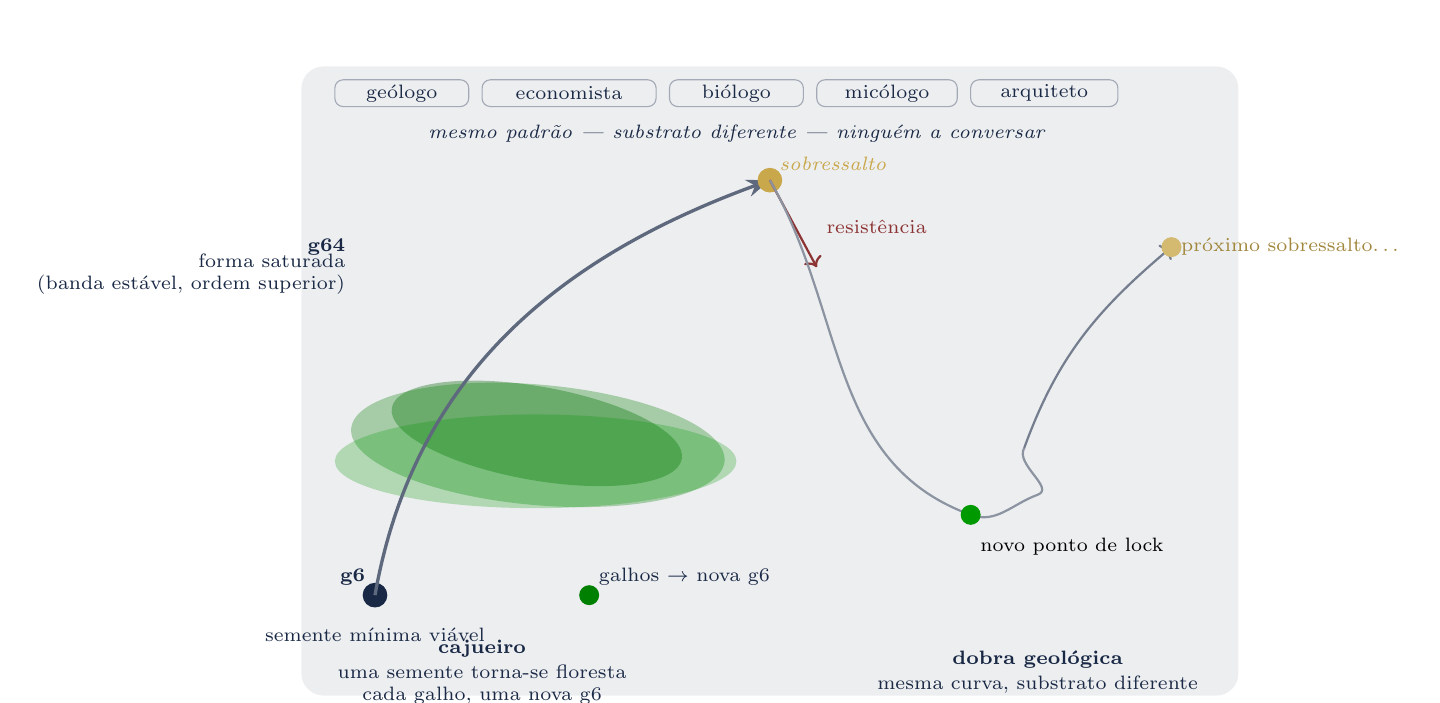
\begin{tikzpicture}[scale=0.85, every node/.style={font=\scriptsize}]
  % Background
  \fill[cajunavy!8, rounded corners=8pt] (-0.5,-1.2) rectangle (13.5,8.2);
  % Discipline chips — individually sized
  \draw[cajunavy!40, rounded corners=3pt] (0.0,7.6) rectangle (2.0,8.0);
  \node[cajunavy] at (1.0,7.8) {geólogo};
  \draw[cajunavy!40, rounded corners=3pt] (2.2,7.6) rectangle (4.8,8.0);
  \node[cajunavy] at (3.5,7.8) {economista};
  \draw[cajunavy!40, rounded corners=3pt] (5.0,7.6) rectangle (7.0,8.0);
  \node[cajunavy] at (6.0,7.8) {biólogo};
  \draw[cajunavy!40, rounded corners=3pt] (7.2,7.6) rectangle (9.3,8.0);
  \node[cajunavy] at (8.25,7.8) {micólogo};
  \draw[cajunavy!40, rounded corners=3pt] (9.5,7.6) rectangle (11.7,8.0);
  \node[cajunavy] at (10.6,7.8) {arquiteto};
  \node[align=center, cajunavy] at (6.0,7.2)
    {\itshape mesmo padrão --- substrato diferente --- ninguém a conversar};
  % Cajueiro canopy
  \fill[green!40!black, opacity=0.35, rotate=-10] (2.5,3.2) ellipse (2.2cm and 0.7cm);
  \fill[green!50!black, opacity=0.30, rotate=-5]  (2.8,2.8) ellipse (2.8cm and 0.9cm);
  \fill[green!60!black, opacity=0.25]              (3.0,2.3) ellipse (3.0cm and 0.7cm);
  % g6 seed
  \filldraw[cajunavy] (0.6,0.3) circle (5pt);
  \node[above left, cajunavy] at (0.6,0.3) {\normalfont\bfseries g6};
  \node[below, cajunavy, align=center] at (0.6,-0.05) {semente mínima viável};
  % g64 label
  \node[left, cajunavy] at (0.3,5.5) {\normalfont\bfseries g64};
  \node[left, cajunavy, align=right] at (0.3,5.1)
    {forma saturada\\(banda estável, ordem superior)};
  % Branch root dot
  \filldraw[green!50!black] (3.8,0.3) circle (4pt);
  \node[above right, cajunavy] at (3.8,0.3) {galhos $\to$ nova g6};
  % Main arc: g6 → overshoot
  \draw[cajunavy!70, very thick, ->, >=Stealth]
    (0.6,0.3) to[out=80, in=200] (6.5,6.5);
  \filldraw[cajugold] (6.5,6.5) circle (5pt);
  \node[above right] at (6.5,6.5) {\textcolor{cajugold}{\itshape sobressalto}};
  % Resistance
  \draw[cajured, thick, ->] (6.5,6.5) -- (7.2,5.2);
  \node[right, cajured] at (7.2,5.8) {resistência};
  % Fold curve
  \draw[cajunavy!50, thick] (6.5,6.5) to[out=-60, in=160] (9.5,1.5)
    to[out=-20, in=200] (10.5,1.8) to[out=20, in=240] (10.3,2.5);
  \filldraw[green!60!black] (9.5,1.5) circle (4pt);
  \node[below right] at (9.5,1.3) {novo ponto de lock};
  % Next overshoot
  \draw[cajunavy!60, thick, ->] (10.3,2.5) to[out=70, in=220] (12.5,5.5);
  \filldraw[cajugold!80] (12.5,5.5) circle (4pt);
  \node[right] at (12.5,5.5) {\textcolor{cajugold!80!black}{próximo sobressalto\ldots}};
  % Bottom captions
  \node[align=center, cajunavy] at (2.2,-0.85)
    {\normalfont\bfseries cajueiro\\[1pt]
     uma semente torna-se floresta\\cada galho, uma nova g6};
  \node[align=center, cajunavy] at (10.5,-0.85)
    {\normalfont\bfseries dobra geológica\\[1pt]
     mesma curva, substrato diferente};
\end{tikzpicture}
\caption{O mesmo padrão generativo manifesta-se em substratos distintos.
  \textbf{g6} (semente mínima viável): condição mínima de estabilidade
  a partir da qual o sistema pode expressar-se. \textbf{g64} (forma saturada):
  expressão máxima estável no limite superior da banda.
  Cada galho que toca o solo torna-se uma nova g6 --- uma nova floresta.}
\label{fig:branches}
\end{figure}

\begin{definicao}[Série g: taxonomia de regimes de estabilidade]\label{def:g-series}
A \textbf{série~g} é um conjunto finito ordenado de rótulos de regime:
\[
  g^{0} < g^{2} < g^{6} < g^{33} < g^{64}.
\]
Cada rótulo $g^{k}$ denomina um regime qualitativo de comportamento de um sistema dm³.
O sobrescrito~$k$ é um índice ordinal, não um expoente. A série não é uma sequência
de números; é uma classificação. Os critérios de atribuição de cada índice são os
seguintes, cada um correspondendo a uma propriedade de estabilidade qualitativamente
distinta do operador $G = U \circ F \circ K \circ C$:

\medskip
\begin{center}
\small
\begin{tabular}{@{}lll@{}}
\toprule
\textbf{Rótulo} & \textbf{Regime} & \textbf{Critério} \\
\midrule
$g^{0}$ & Semente &
  Aplicação de um único operador; sem condição de fechamento. \\[3pt]
$g^{2}$ & Composicional &
  Fechamento com dois operadores; auto-referência mínima ($F$ ativo). \\[3pt]
$g^{6}$ & Escala de ciclo &
  Fechamento do ciclo completo $G$; ciclo-limite $\Gamma$ atingido. \\[3pt]
$g^{33}$ & Equilíbrio suave &
  Índice heurístico de estabilidade (ver Observação abaixo). \emph{Conjectura.} \\[3pt]
$g^{64}$ & Limiar de fase &
  Cobertura completa do espaço de possibilidades: $2^{6} = 64$
  combinações operador--estado. \\
\bottomrule
\end{tabular}
\end{center}

\medskip
\noindent\textbf{Status matemático de $g^{33}$.}
O índice~33 provém da seguinte computação heurística: existem três invariantes que
devem fechar simultaneamente (ortogonalidade, nilpotência dos desvios, colapso
espectral), fornecendo $3! = 6$ ordenamentos; $\lceil \log_{2}(3!)\cdot 4 \rceil =
\lceil 10{,}34\ldots \rceil = 11$; multiplicando por~3 para um critério de robustez
de tripla confirmação obtém-se $3 \times 11 = 33$. O passo ``multiplicar por~3''
reflete uma escolha de projeto --- que três fechamentos independentes são necessários
para estabilidade robusta --- e não é derivado da estrutura de contato. O índice~33
é, portanto, um rótulo motivado, não um teorema. Sua situação matemática é a de uma
\textbf{conjectura}: conjecturamos que sistemas dm³ requerem ao menos 33 ciclos
operacionais para que os três invariantes alcancem fechamento robusto simultâneo.
Isso é identificado como alvo de verificação em aberto no repositório AXLE.

\medskip
\noindent\textbf{Notação de associação.}
A notação $g^{6}\!:\!33$ usada alhures na série \emph{Principia Orthogona} denota
associação, não igualdade: ``o regime de escala de ciclo $g^{6}$ carrega o índice
estrutural~33.'' É um descritor do mesmo tipo que ``simetria D6: 6 eixos'' ou
``rede E8: posto~8.'' Nenhuma identidade algébrica $g^{6} = 33$ é afirmada.
\end{definicao}

\begin{observacao}[Mínimo de multi-órbita e dominância cooperativa]
\provadostamp
Os dois resultados que seguem da teoria multi-órbita são provados
em \cite{GrossiMultiOrbit,GrossiJomo}:
\begin{itemize}
  \item \textbf{Mínimo de multi-órbita.} Para um sistema $\mathcal{S} =
    \{S_1,\dots,S_k\}$ acoplado por raiz comum sob $G$, a classe~g efetiva
    é $g_{\mathrm{ef}}(\mathcal{S}) = \min_i\, g(S_i)$.
    Nenhuma intervenção restrita a um componente não-mínimo pode elevar
    $g_{\mathrm{ef}}$.
  \item \textbf{Dominância cooperativa.} A única estratégia que avança
    $g_{\mathrm{ef}}$ é elevar o componente de menor índice.
    A estratégia cooperativa (elevar o mínimo) domina estritamente toda
    estratégia que maximiza um componente não-mínimo.
\end{itemize}
O limiar $\tau = 2$ é coletivo: um galho em $g^{64}$ inserido numa raiz
em $g^0$ não produz $\tau = 2$. \emph{Sustentável significa que todos os
componentes devem cruzar a linha de chegada.}
\end{observacao}

A Figura~\ref{fig:branches} ilustra esta taxonomia geometricamente: g6 é o ponto
de partida (ponto azul escuro, semente mínima viável); g64 é a copa formada (elipses
verdes, forma saturada). A mesma curva --- a mesma órbita de $G$ --- manifesta-se
em substratos distintos. A Figura~\ref{fig:branches} mostra o que esta série é: não uma progressão
linear de volumes, mas um cajueiro. Cada volume da série B1--B9 é
um galho: uma nova g6, uma nova condição mínima de estabilidade, um novo
campo de potencial onde o mesmo padrão se repete num substrato diferente.

O geólogo vê uma dobra tectônica. O economista vê um ciclo de
sobressalto e resistência. O biólogo vê morfogênese. O micólogo vê rede
miceliar. O arquiteto vê forma emergente. O mesmo padrão. Substratos
diferentes. Ninguém a conversar.

Esta monografia --- e a série que a contém --- é a tentativa de
iniciar essa conversa.

Mas o alcance do princípio não termina no Brasil, nem na Terra. A Teoria das
Transições Generativas ($\dm$) é, na sua essência, uma ciência planetária:
um instrumento para compreender, medir e prever como sistemas evoluem a
partir das condições topológicas do seu espaço de fases --- independentemente
da química específica do planeta onde operam. A cadeia $G = U \circ F \circ K
\circ C$ não pergunta \emph{que moléculas existem aqui}; pergunta \emph{qual
é a topologia do espaço de fases disponível}. É por isso que $\dm$ pode,
em princípio, indicar com precisão quais transições generativas são possíveis
em Marte --- dada a sua atmosfera, a sua geoquímica, a sua pressão --- ou em
Encélado, dadas as suas plumas criovulcânicas e o oceano subsuperficial.
Se decidir mudar-se para Marte, esta monografia oferece a estrutura
matemática para saber o que pode crescer lá, o que pode ser catalisado lá,
e como sobreviver. \textbf{Ciência generativa é ciência planetária.}

Não pretendo continuar todos os galhos. Não viverei para isso. Mas espero
que a \textbf{G6 LLC} --- e os investigadores que encontrarem este trabalho
--- continuem. A estrutura está aqui. A semente está plantada. O que cresce
a seguir é vosso.

% ==================================================================
\chapter{Limitações e Direções Futuras}
\label{cap:limitacoes}

\section{Limitações conhecidas}

\textbf{Subhalos isolados (Encélado).} O tratamento aproxima Encélado
como sistema isolado, desconsiderando o efeito de maré de Saturno e
de Diona. Essa aproximação introduz erro modesto em $r_{c}$ (o raio
crítico) mas não afeta a estrutura algébrica da cadeia.

\textbf{Quimostato vs.\ ribozimas.} A realização ribozímica
(Capítulo~\ref{cap:universalidade}) é demonstrada para sistemas em
estado de fluxo constante. A extensão para sistemas com substratos
variáveis (mais realistas para o mundo de RNA pré-biótico) é objeto
de trabalho futuro.

\textbf{Catálise dinâmica.} O Teorema~\ref{thm:ordem-zeolitas} trata a
estrutura zeolítica como estática. A inclusão de respiração estrutural
sob condições reais de reação é necessária para previsões a temperaturas
extremas.

\textbf{Outros estados brasileiros.} A análise econômica do
Capítulo~\ref{cap:caju-industrial} foca em Ceará, Rio Grande do Norte
e Piauí. Outros estados produtores de caju (Maranhão, Bahia) requerem
ajustes nas estimativas de tonelagem e mão-de-obra.

\section{Direções futuras imediatas}

\textbf{Pedido de patente.} Pedido provisório de patente nos Estados Unidos
sobre o catalisador MCM-22 regulado por boro e o método de controle de
processo via índice~$O$ é a próxima ação concreta, com prazo de 30 dias
a partir da publicação da monografia.

\textbf{Demonstração TRL-4.} Demonstração em escala-piloto de laboratório
em colaboração com a \textbf{Universidade do Estado do Rio de Janeiro (UERJ)}
e, potencialmente, com a \textbf{Universidade Estadual de Campinas (Unicamp)}.
1~kg de catalisador,
reator de 100~mL/h, operando sobre etanol derivado de pseudofruto.

\textbf{Parceria com BNDES e BID.} Apresentação ao BNDES Climate Fund
e ao BID Lab para financiamento da fase de demonstração industrial.

\textbf{Verificação Lean das obrigações abertas.} Fechamento das cinco
obrigações em aberto da Seção~\ref{cap:lean} requer trabalho contínuo
sobre Mathlib4.

\textbf{Extensão Lorentziana.} Conforme descrito no Volume~III, a extensão
do arcabouço para variedades de contato lorentzianas (Beig--Chruściel)
permite tratar horizontes de eventos como dobras de Whitney sobre
superfícies marginalmente capturadas.

% ==================================================================
\appendix
\part{Apêndices}

\chapter{Listagem do Código Lean 4}
\label{ap:lean-codigo}

Conteúdo completo do arquivo \texttt{Cajueiro\_MachineVerified.lean}.
Os arquivos completos da série estão disponíveis no repositório AXLE.

\section*{Estrutura do arquivo}

\begin{lstlisting}[language=lean]
namespace CajueiroVerified
open Real Set Function

-- Constantes certificadas
def tribonacci_constant : R := 1.839090805
def epsilon_zero : R := 1/3

notation "eta" => tribonacci_constant
notation "epsilon_0" => epsilon_zero

-- Axiomas foundationais
axiom tribonacci_gt_one : (eta : R) > 1
axiom tribonacci_upper_bound : (eta : R) < 2
axiom epsilon_zero_positive : (epsilon_0 : R) > 0
axiom epsilon_zero_lt_one : (epsilon_0 : R) < 1

-- Lemas L1-L8 verificados
lemma log_eta_positive : Real.log (eta : R) > 0 :=
  Real.log_pos tribonacci_gt_one

lemma log_epsilon_zero_negative : Real.log (epsilon_0 : R) < 0 :=
  Real.log_neg epsilon_zero_positive epsilon_zero_lt_one

-- Teorema principal: amplificacao Tribonacci
theorem tribonacci_amplification :
  eta ^ (-(Real.log (epsilon_0 : R) / Real.log (eta : R))) > 1 :=
  tribonacci_weighting_gt_one

end CajueiroVerified
\end{lstlisting}

\chapter{Listagem do Código Python}
\label{ap:python-codigo}

Conteúdo central do arquivo \texttt{cajueiro\_simulation.py}.

\begin{lstlisting}[basicstyle=\ttfamily\footnotesize]
#!/usr/bin/env python3
"""
Cajueiro: Simulacao das transicoes generativas.
Catalisis zeolitica + cadeia industrial caju->SAF.
"""

import numpy as np
import matplotlib.pyplot as plt

# Constantes certificadas
EPSILON_ZERO = 1/3
TAU = 2.0
ETA = 1.839090805
KAPPA_STAR = 1.0

def scale_index(x):
    """Indice de escala k(x) = ln(x) / ln(eta)"""
    return np.log(x) / np.log(ETA)

def operator_order_index(zeolite_type, B_fraction=0):
    """Indice O da ordem dos operadores."""
    if zeolite_type == 'ZSM5':
        return 8.0
    elif zeolite_type == 'MCM22':
        base = 0.7
        return base * (1 + 6.3 * B_fraction)

def coke_yield(O):
    """Rendimento de coque em funcao do indice O."""
    return 7.5 * np.exp(-0.65 * O)

def saf_yield_per_ton_ethanol(O):
    """Galoes de SAF/tonelada de etanol."""
    if O > 3:
        return 50 - 5*(O-3)
    return 50 * (O/3)

def cashew_chain_value(M_cashew_apple_kt):
    """Valor da cadeia caju->SAF em USD/ano."""
    ethanol_kt = M_cashew_apple_kt * 0.10
    saf_gal = ethanol_kt * 1000 * 50
    return saf_gal * 4.5
\end{lstlisting}

\chapter{Derivações Detalhadas da Catálise}
\label{ap:cat-derivacoes}

\section{Derivação do índice $O$ a partir do DRIFTS}

O índice $O$ é definido em termos de tempos de aparecimento espectroscópico:
\[
  O = \frac{t_{\text{DEE}}}{t_{\text{EtO}}}, \qquad t_{X} = \text{tempo no qual } I_{X}(t) > 0{,}1 \cdot \max_{t} I_{X}(t).
\]
A integração das bandas $I_{X}(t)$ usa janelas de 30~cm$^{-1}$ centradas
nas frequências literatura para cada espécie (etóxido em 2975, 2930,
2870, 1450, 1390~cm$^{-1}$; DEE em 1115~cm$^{-1}$).

\section{Conexão com a não-comutatividade}

Em uma zeólita com sítios ácidos distribuídos em superfície de poro
$\Sigma$, a ação dos operadores em uma molécula entrante é:
\[
  K(\phi_{0}) = \text{constrição pela boca do poro}, \qquad
  F(\phi_{0}) = \text{dobramento conformacional}.
\]
A não-comutatividade $[K,F] \ne 0$ implica
$K \circ F (\phi_{0}) \ne F \circ K (\phi_{0})$. O DRIFTS resolve qual
das duas ordens ocorre em tempo real.

\chapter{Dados da Indústria do Caju}
\label{ap:caju-dados}

\section{Tonelagens e geografia}

\begin{tabular}{lrrr}
\toprule
\textbf{Estado} & \textbf{Produção (kt)} & \textbf{Empregados} & \textbf{Cooperativas} \\
\midrule
Ceará               & 65  & 110\,000 & Cionorte e outras \\
Rio Grande do Norte & 30  &  60\,000 & Cocajupi e outras \\
Piauí               & 20  &  30\,000 & Várias \\
Outros              &  5  &  10\,000 & --- \\
\midrule
\textbf{Total Brasil} & 120 & 210\,000 & --- \\
\bottomrule
\end{tabular}

\section{Composição do pseudofruto}

\begin{tabular}{lr}
\toprule
\textbf{Componente} & \textbf{Fração mássica} \\
\midrule
Água                       & 85--87\% \\
Açúcares (glicose+frutose) & 8--12\% \\
Polifenóis (taninos)       & 0,5--1\% \\
Pectina                    & 0,5--1\% \\
Outros                     & 1--2\% \\
\bottomrule
\end{tabular}

\chapter{Bibliografia Completa}
\label{ap:bibliografia}

Veja a lista de referências ao final do volume.

% ──────────────────────────────────────────────────────────────────
\backmatter
\begin{thebibliography}{99}

\bibitem{Arnold1985} V.~I. Arnol'd, A.~N. Varchenko, S.~M. Gusein-Zade,
  \emph{Singularities of Differentiable Maps, Volume 1.}
  Birkh\"auser, Boston, 1985.

\bibitem{Eliashberg1992} Y. Eliashberg, ``Contact 3-manifolds twenty years since J. Martinet's work,''
  \emph{Ann. Inst. Fourier} \textbf{42} (1--2), 165--192 (1992).

\bibitem{Etnyre2003} J.~B. Etnyre, ``Introductory lectures on contact geometry,''
  in \emph{Topology and Geometry of Manifolds}, AMS, 2003.

\bibitem{Geiges2008} H. Geiges, \emph{An Introduction to Contact Topology}.
  Cambridge Studies in Advanced Mathematics 109. Cambridge Univ. Press, 2008.

\bibitem{Gray1959} J.~W. Gray, ``Some global properties of contact structures,''
  \emph{Ann. of Math.} (2) \textbf{69}, 421--450 (1959).

% ---- Principia Orthogona / dm³ — todos os DOIs são DOIs de conceito Zenodo
%      (resolvem sempre para a versão mais recente do depósito) ----

\bibitem{Grossi2026I} P.~N. Grossi, \emph{Principia Orthogona, Vol.~I}.
  Zenodo: \href{https://doi.org/10.5281/zenodo.19117399}{10.5281/zenodo.19117399} (2026).
  CC BY 4.0.

\bibitem{Grossi2026II} P.~N. Grossi, \emph{Principia Orthogona, Vol.~II: Realização de Contato}.
  Zenodo: \href{https://doi.org/10.5281/zenodo.20159456}{10.5281/zenodo.20159456} (2026).
  CC BY 4.0.

\bibitem{GrossiMultiOrbit} P.~N. Grossi, \emph{Biological Transitions as Multi-Agent Realisations
  of the Generative Operator Pipeline in TOGT: A Fruit-Fly Connectome Toy Model}.
  Zenodo: \href{https://doi.org/10.5281/zenodo.19210136}{10.5281/zenodo.19210136} (2026).

\bibitem{GrossiTOGT} P.~N. Grossi, \emph{Contact-Geometric Theory of Generative Transitions:
  Mathematical Foundations, Contact Realization, Seven Proofs of the Tribonacci Constant,
  and Applications to Nuclear Matter}.
  Zenodo: \href{https://doi.org/10.5281/zenodo.20682933}{10.5281/zenodo.20682933} (2026).
  CC BY 4.0.

\bibitem{GrossiAlterna} P.~N. Grossi, \emph{Alternating Vanishing Theorem and
  Contact-Geometric Integrability Tower}.
  Zenodo: \href{https://doi.org/10.5281/zenodo.20710023}{10.5281/zenodo.20710023} (2026).

\bibitem{GrossiOrtho} P.~N. Grossi, \emph{Topological Orthogenesis and the Universality Class
  of Generative Transitions}.
  Zenodo: \href{https://doi.org/10.5281/zenodo.20849637}{10.5281/zenodo.20849637} (2026).
  CC BY 4.0.

\bibitem{GrossiSCITBI} P.~N. Grossi, \emph{dm$^{3}$ Contact-Geometric Prediction of
  Neurological Recovery: Preliminary Analysis of Published NSCISC, TBIMS, and TRACK-TBI
  Longitudinal Data}.
  Zenodo: \href{https://doi.org/10.5281/zenodo.20802299}{10.5281/zenodo.20802299} (2026).
  CC BY 4.0.

\bibitem{GrossiCatalise} P.~N. Grossi, \emph{Operator Firing Order as the Missing Mechanism
  in Ethanol-to-Hydrocarbon Selectivity}.
  Zenodo: \href{https://doi.org/10.5281/zenodo.20563363}{10.5281/zenodo.20563363} (2026).

\bibitem{GrossiEnceladus} P.~N. Grossi, \emph{Generative Transitions in Cryovolcanic Systems:
  A Principia Orthogona Analysis of the Enceladus Plume}.
  Zenodo: \href{https://doi.org/10.5281/zenodo.20779067}{10.5281/zenodo.20779067} (2026).

\bibitem{GrossiTEFL} P.~N. Grossi, \emph{Nested Infinities in the Language Classroom:
  A Contact-Geometric Model of Fluency, the ZPD, and the L2 Teacher Advantage}.
  Zenodo: \href{https://doi.org/10.5281/zenodo.20719398}{10.5281/zenodo.20719398} (2026).
  CC BY 4.0.

\bibitem{GrossiJomo} P.~N. Grossi, \emph{Positional Dominance in Network Games:
  Equilibrium Conditions for Strategic Abstention from Velocity Competition}.
  Zenodo: \href{https://doi.org/10.5281/zenodo.21013066}{10.5281/zenodo.21013066} (2026).

\bibitem{Khawaja2025} N. Khawaja \emph{et al.}, ``Mass spectrometric analysis of the Enceladus plume,''
  \emph{Nature Astronomy} \textbf{9}, 1662--1671 (2025).

\bibitem{Russell} M.~J. Russell, A.~J. Hall, ``The emergence of life from iron monosulphide bubbles at a submarine hydrothermal redox and pH front,''
  \emph{J.~Geol.~Soc.} \textbf{154}, 377--402 (1997).

\bibitem{Sojo} V. Sojo, A. Pomiankowski, N. Lane, ``A bioenergetic basis for membrane divergence in archaea and bacteria,''
  \emph{PLoS Biol.} \textbf{12}, e1001926 (2014).

\bibitem{Joyce} G.~F. Joyce, \emph{The RNA world}, in: R.~F. Gesteland, J.~F. Atkins (eds.),
  \emph{The RNA World}, Cold Spring Harbor Laboratory Press, 1993.

\bibitem{Sousa2014} Z. Sousa \emph{et al.}, ``Selectivity in ethanol conversion over HZSM-5 and HMCM-22,''
  \emph{Microporous Mesoporous Mater.} (2014). [Completar volume e páginas antes da submissão.]

\bibitem{Sousa2023} Z. Sousa \emph{et al.}, ``Dealuminated and delaminated variants in ETH catalysis,''
  \emph{Catalysis Today} (2023). [Completar volume e páginas antes da submissão.]

\bibitem{Halle1978} F. Hall\'e, R.~A.~A. Oldeman, P.~B. Tomlinson,
  \emph{Tropical Trees and Forests: An Architectural Analysis}.
  Springer-Verlag, Berlin, 1978.

\bibitem{Thom1975} R. Thom, \emph{Structural Stability and Morphogenesis:
  An Outline of a General Theory of Models}.
  Addison-Wesley, Reading, MA, 1975. [Trad. inglesa de \emph{Stabilité structurelle et morphogénèse}, 1972.]

\bibitem{Prigogine} I. Prigogine, \emph{From Being to Becoming}.
  W.~H. Freeman, 1980.

\bibitem{England} J. England, ``Statistical physics of self-replication,''
  \emph{J. Chem. Phys.} \textbf{139}, 121923 (2013).

\bibitem{Hatcher} A. Hatcher, \emph{Algebraic Topology}.
  Cambridge Univ. Press, 2002.

\end{thebibliography}

% ==================================================================
\chapter*{Nota aos Revisores: Terminologia e Ortografia}
\addcontentsline{toc}{chapter}{Nota aos Revisores: Terminologia e Ortografia}
% ==================================================================

Algumas escolhas terminológicas desta monografia diferem das formas
previstas pelo Acordo Ortográfico de 2009. As divergências são
deliberadas e têm justificativa na tradição matemática brasileira.

\medskip
\textbf{``Conjectura'' (e não ``conjetura'').}
O Acordo Ortográfico de 2009 suprime o~\textit{c} em palavras
como \emph{conjectura} e \emph{conjectural}. Contudo, a cultura
matemática brasileira --- incluindo publicações do IMPA, da SBM
e de periódicos internacionais de língua portuguesa --- preserva
a grafia histórica \textbf{conjectura} por décadas de uso consagrado.
Mantemos essa grafia ao longo desta monografia.

\medskip
\textbf{``Contactomorfismo'' / ``contactomorfa'' (com \textit{c}).}
O Acordo Ortográfico prevê \emph{contacto} $\to$ \emph{contato}.
Na literatura de geometria diferencial, contudo, o termo técnico
\textbf{contactomorfismo} (\emph{contactomorphism}) preserva
o~\textit{c} para manter a legibilidade da raiz latina e a
correspondência direta com a terminologia internacional.
Usamos \textbf{contactomorfa} (e não ``contatomórfica'') por essa razão.

\medskip
\textbf{``Cúspide'' (substantivo feminino).}
Adotamos \emph{a cúspide} (feminino) em conformidade com a tradição
geométrica e dicionarística portuguesa. Em contexto de teoria das
catástrofes, ``a cúspide $A_2$'' é a singularidade de codimensão~2
na classificação de Whitney--Thom.

\medskip
\textbf{``Grosso modo'' (sem hífen).}
A locução adverbial latina \emph{grosso modo} não leva hífen em
português moderno. Usamos sempre a forma sem hífen.

\end{document}
